\section{Proofs of Theoretical Claims for \ours}
\label{sec:appx-proofs}

\begin{theorem}
	(Universal Approximation of Neural Operators):
	Given a compact set $\mathcal{K} \subset \mathcal{H}$ and a continuous nonlinear operator $\mathcal{G}: \mathcal{K} \rightarrow \mathcal{Y},$ for every $\epsilon > 0$ there exists a parameter set $\theta$ of the neural operator $\mathcal{G}_\theta$, such that:
	\[
		\sup _{f \in \mathcal{K}}\left\|\mathcal{G}(f)-\mathcal{G}_\theta(f)\right\|_{\mathcal{Y}}<\varepsilon .
	\]
\end{theorem}

\begin{proof}
	This theorem directly follows from the universal approximation theorem for operators stated and proven by ~\cite{kovachki2023neural}. Neural operator architectures, such as the Fourier Neural Operator and DeepONet, have been rigorously proven to possess universal approximation capabilities in appropriate Banach spaces.
	
	Specifically, the proof leverages the density of neural network-generated basis functions in function spaces, using the Stone-Weierstrass theorem to approximate continuous operators with arbitrary precision. Given that COMPOL leverages neural operators with additional latent aggregation mechanisms, the universal approximation capacity remains unaffected, as these aggregation mechanisms are continuous mappings and thus preserve the universal approximation property.
\end{proof}

\begin{theorem}
	(Convergence of Iterative Latent Feature Transformation):
	Consider the iterative latent transformation defined by:
	\[
		v_l^m=\Phi_l^m\left(v_{l-1}^m, z_{l-1}\right), \quad z_{l-1}=\mathcal{A}\left(\left\{v_{l-1}^m\right\}_{m=1}^M\right) .
	\]
	If $\Phi_l^m$ and $\mathcal{A}$ are Lipschitz continuous with Lipschitz constants $L_{\Phi}$ and $L_{\mathcal{A}}$, respectively, and if $L_{\Phi}L_{\mathcal{A}} <1$, then the iterative scheme converges to a unique fixed point.
\end{theorem}

\begin{proof}
	By the Banach fixed-point theorem, convergence to a unique fixed point is guaranteed if the combined iterative mapping is a contraction. Define the combined operator $\mathcal{T}$ such that:
	\[
		\mathcal{T}(\mathbf{v}):=\Phi(\mathbf{v}, \mathcal{A}(\mathbf{v})), \quad \mathbf{v}:=\left\{v^m\right\}_{m=1}^M .
	\]
	
	For  in the latent space, we have:
	\[
		\|\mathcal{T}(\mathbf{v})-\mathcal{T}(\mathbf{w})\| \leq L_{\Phi}\|\mathbf{v}-\mathbf{w}\|+L_{\Phi} L_{\mathcal{A}}\|\mathbf{v}-\mathbf{w}\|=L_{\Phi}\left(1+L_{\mathcal{A}}\right)\|\mathbf{v}-\mathbf{w}\| .
	\]
	If $L_{\Phi}\left(1+L_{\mathcal{A}}\right)<1$, $\mathcal{T}$ is is a contraction, and thus by the Banach fixed-point theorem, the iterative procedure converges to a unique fixed point in the latent representation.
\end{proof}

\begin{theorem}
	 (Stability of Aggregation Mechanisms):
	The aggregation mechanism $\mathcal{A}(\cdot)$, either recurrent-based or attention-based, preserves stability in latent space representation provided that all internal parameters remain bounded and activations are Lipschitz continuous. 
\end{theorem}

\begin{proof}
	Aggregation mechanisms such as RNNs and attention modules can be expressed as compositions of linear transformations and Lipschitz continuous nonlinearities (e.g., sigmoid, tanh, softmax). Since compositions of Lipschitz continuous functions with bounded parameters remain Lipschitz continuous and bounded, the aggregation mechanism:
	\[
		z=\mathcal{A}\left(v^1, v^2, \ldots, v^M\right)
	\]
	remains stable. Specifically, given Lipschitz continuity of all intermediate functions with constants $L_i$, we have:
	\[
		\|\mathcal{A}(\mathbf{v})-\mathcal{A}(\mathbf{w})\| \leq\left(\prod_i L_i\right)\|\mathbf{v}-\mathbf{w}\|,
	\]
	indicating the stability of aggregation as long as all parameters and operations remain bounded and well-conditioned.
\end{proof}


\newpage
\section{Adapting \ours to Alternative Neural Operator Backbones}
\label{sec:appx-adapting}

COMPOL enhances neural operators by explicitly modeling latent interactions among multiple physical processes. Given $M$ coupled processes, latent features at layer $l$ are updated as:
\begin{equation}
	v_l^{m}(x) = h_l^{m}\left(v_{l-1}^{m}(x), z_{l-1}(x)\right),\quad m=1,\dots,M,\notag
\end{equation}
where the latent aggregation $z_{l-1}(x)$ is:
\begin{equation}
	z_{l-1}(x) = \mathcal{A}\left(v_{l-1}^{1}(x), v_{l-1}^{2}(x), \dots,\notag v_{l-1}^{M}(x)\right).
\end{equation}

\subsection{DeepONet + \ours}
Original DeepONet~\citep{lu2021learning} approximates an operator $G: f \mapsto g$:
\[
	G(f)(y) \approx \sum_{j=1}^p b_j(f) \cdot t_j(y),
\]
where $b_j$ and $t_j$ represent branch and trunk neural networks. COMPOL introduces latent aggregation $z$ to enhance interactions between the branch and trunk networks, explicitly modeling their latent interdependencies:
\begin{itemize}
	\item Aggregate branch-trunk latent features:
	\[
		z=\mathcal{A}\left(b_j(f), t_j(y)\right)
	\]
	\item Modified DeepONet prediction
	\[
		G(f)(y) \approx \sum_{j=1}^p b_j^{\prime}(f, z) \cdot t_j^{\prime}(y, z)
	\]
\end{itemize}

\subsection{GNO + \ours}
Graph Kernel Network (GKN) has been adopted by existing works for partial differential equations~\cite{li2020neural}, while the evolution of latent features is typically local-each update depends only on the current layer's hidden state and neighborhood structure. Therefore, such a design overlooks the rich temporal evolution and accumulated semantics across layers. By contrast, COMPOL introduces a layer-wise aggregated latent representation $z_l$ that synthesizes information from all prior hidden states $\left\{v_j^{(m)}\right\}_{j=0}^{l-1}$ across all processes $m$. Formally, the adapted message passing operator is given as
\begin{align}
	v^{(m)}_{l+1}(x) = \sigma\Bigg(
	W v^{(m)}_t(x) +
	\frac{1}{|\mathcal{N}(x)|} \sum_{y \in \mathcal{N}(x)} \kappa_\phi(e(x, y)) v^{(m)}_l(y) + W_z z_t(x)\notag
	\Bigg),
\end{align}
where $W_z$ represents a learnable matrix enforcing a linear transformation to align dimensions of $z_l(x)$ with $W v^{(m)}_l(x)$. Such an adaptation for GKN allows the message passing at each spatial location to dynamically adjust its representation based on both the multi-process coupling and the full history of the model's latent dynamics. 

\subsection{LNO + \ours}
Low-rank Neural Operator (LNO)~\citep{kovachki2023neural} approximates operators via low-rank decompositions:
\[
	v_l(x)=\sum_{k=1}^K \alpha_k(x) \beta_k(x)
\]
where $\alpha_k, \beta_k$ represent latent low-rank features. COMPOL aggregation explicitly models inter-rank interactions:
\begin{itemize}
	\item Aggregation step:
	\[
		z_{l-1}(x)=\mathcal{A}\left(\alpha_k(x), \beta_k(x)\right).
	\]
	\item Modified LNO:
	\[
		v_l(x)=\sum_{k=1}^K \alpha_k^{\prime}\left(x, z_{l-1}(x)\right) \beta_k^{\prime}\left(x, z_{l-1}(x)\right).
	\]
\end{itemize}

\subsection{Transformer-based Neural Operators (\eg Transolver) + \ours}
Transformer-based neural operators perform positional self-attention:
\[
	v_l\left(x_i\right)=\operatorname{Attention}\left(Q_i, K_j, V_j\right), \quad Q_i=Q\left(v_{l-1}\left(x_i\right)\right), K_j=K\left(v_{l-1}\left(x_j\right)\right), V_j=V\left(v_{l-1}\left(x_j\right)\right)
\]
To integrate COMPOL into transformer-based neural operator learning frameworks, we introduce an additional COMPOL aggregates across processes before applying positional attention.

\paragraph{Per-process latent feature aggregation (COMPOL step)} Given multiple processes $m=1, \ldots, M$, latent representations at layer $l-1 \text { are } v_{l-1}^m(x)$. First, compute aggregated latent representation across processes via attention:
\[
	z_{l-1}(x)=\mathcal{A}\left(v_{l-1}^1(x), v_{l-1}^2(x), \ldots, v_{l-1}^M(x)\right) .
\]

\paragraph{Positional Attention enhanced by aggregated latent representation} Next, perform standard positional transformer attention at position $x_i$, but now augment it with the aggregated latent representation $z_{l-1}\left(x_i\right)$:
\begin{itemize}
	\item Compute positional queries, keys, values:
	\[
		Q_i{ }^{\prime}=Q^{\prime}\left(v_{l-1}\left(x_i\right), z_{l-1}\left(x_i\right)\right), K_j^{\prime}=K^{\prime}\left(v_{l-1}\left(x_j\right), z_{l-1}\left(x_j\right)\right), V_j^{\prime}=V^{\prime}\left(v_{l-1}\left(x_j\right), z_{l-1}\left(x_j\right)\right) .
	\]
	\item Apply enhanced positional attention:
	\[
		v_l\left(x_i\right)=\sum_j \alpha^{\prime}_{ij} V_j^{\prime}, \quad \text { where } \quad \alpha^{\prime}_{ij}=\frac{\exp \left(Q_i{ }^{\prime} \cdot K_j{ }^{\prime} / \sqrt{d_k{ }^{\prime}}\right)}{\sum_j \exp \left(Q_i{ }^{\prime} \cdot K_j{ }^{\prime} / \sqrt{d_k{ }^{\prime}}\right)} .
	\]
\end{itemize}
Here, the latent aggregation $z_{l-1}\left(x_i\right)$ explicitly modulates the positional attention, guiding the attention mechanism to better capture multi-physics process interactions.

\newpage
\section{Details of Synthetic Multi-Physics Datasets}
\label{sec:appx-synt}

\paragraph{1-D Lotka-Volterra Equation}The 1-D reaction-diffusion Lotka-Volterra system models predator-prey population dynamics through coupled partial differential equations:
\begin{equation}
	\begin{cases}
		\frac{\partial u}{\partial t} = D_u\nabla^2 u + au - buv \notag \\
		\frac{\partial v}{\partial t} = D_v\nabla^2 v + cuv -dv \notag
	\end{cases}
\end{equation}
The system combines spatial diffusion (coefficients $D_u$ and $D_v$) with population interactions through reaction terms, generating complex spatio-temporal patterns. We study this system using a one-dimensional Gaussian Random Field initialization (length-scale $l=0.1$, amplitude $\sigma=1$) with periodic boundary conditions and uniform interaction parameters ($a=b=c=d=0.01$) and uniform diffusion coefficients ($D_u=D_v=0.01$) to examine the fundamental dynamics.

%\paragraph{1-D Coupled Burgers' Equation} The coupled Burgers' equation models the evolution of two interrelated spatio-temporal variables, $u(x,t)$ and $v(x,t)$, through a pair of interconnected equations:
%
%\begin{equation}
%	\begin{cases}
%		\frac{\partial u}{\partial t} = -u\frac{\partial u}{\partial x} - v\frac{\partial u}{\partial x} + \nu\nabla^2 u \notag \\
%		\frac{\partial v}{\partial t} = -v\frac{\partial v}{\partial x} - u\frac{\partial v}{\partial x} + \nu\nabla^2 v \notag 
%	\end{cases}
%\end{equation}
%The system's behavior is governed by the viscosity coefficient $\nu$, which controls diffusion strength. The equations are coupled through advection terms $v\frac{\partial u}{\partial x}$ and $u\frac{\partial v}{\partial x}$, enabling the system to model fluid interactions, wave propagation, and transport processes in multi-component systems.
%At low viscosity values ($\nu=0.1$ in our setup), the nonlinear advection terms become dominant, potentially producing shock waves. Using Gaussian pulse initial conditions with Dirichlet boundary conditions, we aimed to map these initial states to system solutions at time $T=2$.

\paragraph{1-D Belousov-Zhabotinsky Equations} 
The Belousov-Zhabotinsky (BZ) reaction is a classical example of nonlinear chemical oscillations and pattern formation in reaction-diffusion systems ~\citep{taylor2002mechanism}. The coupled BZ equations describe a reaction-diffusion process with three reactants $u(x,t)$, $v(x,t)$, and $w(x,t)$:

\begin{equation}
	\begin{cases}
		\frac{\partial u}{\partial t} = \epsilon_1 \nabla^2 u + u + v - uv - u^2 \\
		\frac{\partial v}{\partial t} = \epsilon_2 \nabla^2 v + w - v - uv \\
		\frac{\partial w}{\partial t} = \epsilon_3 \nabla^2 w + u - w \notag
	\end{cases}
\end{equation}

where we set $\epsilon_1 = 1 \times 10^{-2}$, $\epsilon_2 = 1 \times 10^{-2}$, and $\epsilon_3 = 5 \times 10^{-3}$ and simulated the system from $t=0$ to $t=0.5$. The system exhibits complex spatiotemporal patterns due to the nonlinear coupling between the chemical species through terms like $uv$ and $u^2$. Initial conditions $u(x,0)$, $v(x,0)$, and $w(x,0)$ were generated using 1D Gaussian Random Field of Gaussian kernel and periodic boundary with correlation length being $0.03$ respectively. The equations were solved numerically using the fourth-order exponential time-differencing Runge-Kutta method (ETDRK4) with a resolution of $1024$, subsequently subsampled to create datasets with resolution $256$. 


\paragraph{2-D Grey-Scott Equation} The Gray-Scott equations model pattern formation in chemical reactions through coupled partial differential equations:
\begin{equation}
	\begin{cases}
		\frac{\partial u}{\partial t} = D_u\nabla^2 u - uv^2 + F(1-u) \notag \\
		\frac{\partial v}{\partial t} = D_v\nabla^2 v + uv^2 + (F+k)v \notag
	\end{cases}
\end{equation}
The system tracks two chemical species: an activator ($u$) and an inhibitor ($v$). Their evolution is governed by diffusion (coefficients $D_u$ and $D_v$), an autocatalytic reaction ($uv^2$), and regulatory mechanisms through feeding rate $F$ and removal rate $k$. The interplay of these processes generates diverse patterns like spots and stripes, with their characteristics determined by the system parameters.
To study these pattern-forming dynamics, we examine the system's evolution from a two-dimensional Gaussian Random Field initial condition to time $T=20$, observing how perturbations develop into organized spatial structures. For all experiments reported, we employed the Gray-Scott system parameters $D_u=0.12$, $D_v=0.06$, $F=0.054$, and $k=0.063$.


\newpage
\section{Details of Multiphase Flow Problem}
\label{sec:appx-mf}

Multiphase flow describes fluid mixtures moving simultaneously —a process critical for underground resource management, including oil and gas extraction, geological carbon storage, and nuclear waste disposal. We study oil-water two-phase flow using GEOS\footnote{\href{https://github.com/GEOS-DEV/GEOS}{https://github.com/GEOS-DEV/GEOS}} on a 2D domain with water injection and oil extraction points on opposite boundaries. The domain permeability ranges from $1mD$ to $1000mD$, sampled based on the fractal distribution ~\citep{tang2021fractal}. Our dataset includes 1024 scenarios with varying boundary configurations, each simulated for 15 timesteps over $7.5\times10^6$ seconds. The goal is to predict the evolution of phase pressure ($P_p$) and saturation ($S_p$) distributions. Section \ref{sec:appx-mf} provides detailed specifications.

Multiphase flow is the simultaneous movement of two or more phases which is one of the most dominant subsurface processes for oil and gas extraction, transport of pollutants in subsurface environments, and geological carbon storage. Due to the presence of multiple phases, considerable complications are always encountered in describing and quantifying the nature of the flow. Here we present a 2D multiphase case of an underground oil-water two-phase flow. 
The components $\alpha$ (water) and $\beta$ (oil) of the multiphase flow fulfill the mass conservation equation:
\begin{equation}
	\begin{cases}
		\frac{\partial M^\alpha}{\partial t} = -\nabla \cdot \left( \mathbf{F}^\alpha_{\text{a}} + \mathbf{F}^\alpha_{\text{d}} \right) + q^\alpha \notag \\
		
		\frac{\partial M^\beta}{\partial t} = -\nabla \cdot \left( \mathbf{F}^\beta_{\text{a}} + \mathbf{F}^\beta_{\text{d}} \right) + q^\beta \notag
	\end{cases}
\end{equation}
where $\mathbf{F}^\alpha_{\text{a}}$ and $\mathbf{F}^\beta_{\text{a}}$ are the advective mass flux, $\mathbf{F}^\alpha_{\text{d}}$ and $\mathbf{F}^\beta_{\text{d}}$ are the diffusive mass flux, $q^\alpha$ and $q^\beta$ are the source or sink terms, and $\M^\alpha$ and $\M^\beta$ are the mass accumulation terms given by
\begin{equation}
	\begin{cases}
		M^{\alpha} = \phi \sum_{p} S_{p} \rho_{p} X_{p}^{\alpha} \notag \\
		M^{\beta} = \phi \sum_{p} S_{p} \rho_{p} X_{p}^{\beta} \notag
	\end{cases}
\end{equation}
In the mass accumulation terms, $\phi$ is the porosity, $S_{p}$ is the saturation of phase $p$, $X_{p}^{\alpha}$ or $X_{p}^{\beta}$ is the mass
fraction of component $\alpha$ or $\beta$ in phase $p$, and $\rho_{p}$ is the density of phase $p$.
In the scenarios of subsurface oil-water two-phase flow, $\mathbf{F}^\alpha_{\text{d}}$ and $\mathbf{F}^\beta_{\text{d}}$ including molecular diffusion and hydrodynamic dispersion are often negligible when compared to $\mathbf{F}^\alpha_{\text{a}}$ and $\mathbf{F}^\beta_{\text{a}}$. For simplicity, we don't include diffusion terms in our simulations. And the advective mass flux equations of component $\alpha$ and $\beta$ are
\begin{equation}
	\begin{cases}
		\mathbf{F}^\alpha \big|_{\text{a}} = \sum_p X_p^\alpha \rho_p \mathbf{u}_p \notag \\
		\mathbf{F}^\beta \big|_{\text{a}} = \sum_p X_p^\beta \rho_p \mathbf{u}_p \notag
	\end{cases}
\end{equation}
Here, $\mathbf{u}_p$ is the Darcy velocity of phase $p$ defined as follows:
\begin{equation}
	\mathbf{u}_p = -k \left( \nabla P_p - \rho_p \mathbf{g} \right) k_{rp} / \mu_p \notag
\end{equation}
where $k$ is the absolute permeability tensor, $P_p$ is the fluid pressure of phase $p$, $\mathbf{g}$ is the gravitational acceleration, $k_{rp}$ is the relative permeability of phase $p$, and $\mu_p$ is the viscosity of phase $p$. The fluid pressure for wetting phase $P_w$ or non-wetting phase $P_n$ is 
\begin{equation}
	P_n = P_w + P_c \notag
\end{equation}
where $P_c$ is the capillary pressure.

In this study, the simulation is performed on GEOS which is an open-source multiphysics simulator. To simulate the oil-water two-phase flow, water is injected into a 2D ($64\times64$ grids) domain from two randomly placed sources on the left boundary. And at the same, oil is produced from two randomly placed sinks on the right boundary. The permeability fields ($k_x$=$k_y$) are generated using a fractal algorithm with $k_{min}=1mD$, $k_{max}=1000mD$, and $k_{base}=100mD$. And the porosity field is generated by the following correlation:
\begin{equation}
	\phi = \left( \frac{k_x}{1 \times 10^{-15} \times 0.0009} \right)^{\frac{1}{4.0001}} \times \frac{1}{100} \notag
\end{equation}
For the 1024 cases in the dataset, we keep all other conditions identical and only change the locations of sources and sinks. For each case, the multiphysics solver is performed every $5\times10^5$ seconds for 15 times and the whole simulation has a time duration of $7.5\times10^6$. During the simulation, the spatial and temporal results of phase pressure and phase saturation are stored at every time step which makes the dimension of the dataset to be $1024\times15\times64\times64\times2$. Our objective here is to learn the mapping from an earlier spatial distribution of $S_p$ and $P_{p}$ to that of a later time step.

\newpage
\section{Details of Thermo-Hydrolic-Mechanics Problem}
\label{sec:appx-thm}

The coupled thermo-hydro-mechanical (THM) processes in porous media and fractured rock are associated with a wide range of applications including geothermal energy extraction, induced seismicity from fluid injection, reservoir stimulation, and nuclear water disposal in subsurface. All the problems involve strong coupling among pressure diffusion, heat transfer, and change of in-situ stress and rock deformation. Here we present a 2D THM case adapted from the 1D thermo-hydro-mechanical problem presented in ~\cite{gao2020three}. 
The governing equations (momentum balance equation, fluid mass balance equation, and heat transfer equation) of THM problems can be derived from the thermo-poroelasticity theory of porous and permeable rock.
\begin{equation}
	\begin{aligned}
		& G u_{i,jj} + \frac{G}{1 - 2\nu} u_{j,ji} - \alpha p_{,i} - \frac{2G \alpha^T_m (1 + \nu)}{3(1 - 2\nu)} T_{i} + F_i = 0, \\
		& \frac{\partial p}{\partial t} = M \left[ \frac{k}{\mu} p_{jj} - \alpha \frac{\partial \varepsilon_{kk}}{\partial t} + \left( \alpha \alpha^T_m + \phi_0 (\alpha^T_f - \alpha^T_m) \right) \frac{\partial T}{\partial t} \right] + \gamma, \\
		& \frac{\partial T}{\partial t} = \frac{1}{\rho_t C_t} (\kappa^T T_i)_i - \frac{\rho_f C_f}{\rho_t C_t} v_i T_{i}.
	\end{aligned}
\end{equation}
where $G$ is the shear modulus of the solid skeleton, $\nu$ is the Poisson’s ratio, $\alpha $ is the Biot’s coefficient, $p_i$ is the pore pressure gradient on $i$ direction, $\alpha^T_m$ is the thermal expansion coefficient of the porous media, $T_i$ is the temperature gradient on $i$ direction ,$F_i$ is the body force term on $i$ direction, $\frac{\partial p}{\partial t}$ is the time change rate of pore pressure, $M$ is the Biot modulus, $\frac{k}{\mu}$ is the hydraulic conductivity, $\frac{\partial \varepsilon_{kk}}{\partial t}$ is the time rate change of volumetric strain, $\phi_0$ is the initial porosity, $\alpha^T_f$ is the thermal expansion coefficient of the fluid, $\frac{\partial T}{\partial t}$ is the time rate change of temperature, $\gamma$ is the source or sink term of the fluid, $\rho_t$ is the total density of the porous media, $\mathit{C_t}$ is the total heat capacity, $\kappa^T$ is the thermal conductivity tensor, $\rho_f$ is the fluid density, $\mathit{C_f}$ is the fluid heat capacity, and $\mathit{v_i}$ is the fluid velocity component.

In this study, the simulation is performed on GEOS which is an open source multiphysics simulator. To simulate pressure diffusion, heat transfer, and change of in-situ stress and rock deformation, a 2D ($64\times64$ grids) domain on XY plane with actual size of 32 m by 32 m and thickness of 0.5 m in Z direction is employed. For each simulation, a random temperature field with a range of 273 to 323 K and random permeability fields are mapped to the grid. The permeability fields ($k_x$=$k_y$) are generated using a fractal algorithm with $k_{min}=10\, D$, $k_{max}=200\, D$, and $k_{base}=50\, D$.

For the 1250 cases in the dataset, we keep all other conditions identical and only change the realizations of temperature and permeability fields. For each case, the multiphysics solver is performed 12 times as $2\times500$ seconds, $4\times1250$ seconds, $4\times2250$ seconds, and $2\times4000$ seconds consecutively and the whole simulation has a time duration of $2.3\times10^4$ seconds. During the simulation, the spatial and temporal results of pore pressure, strain, and temperature are stored at every time step which makes the dimension of the dataset to be $1250\times12\times64\times64\times3$. Our objective here is to learn the mapping from an earlier spatial distribution of pore pressure, strain, and temperature to that of a later time step.


\newpage
\section{Predictions of \ours and Baseline Models vs. Ground Truth}
\label{sec:pred_ground}

\begin{figure*}[!htbp]
	\centering
	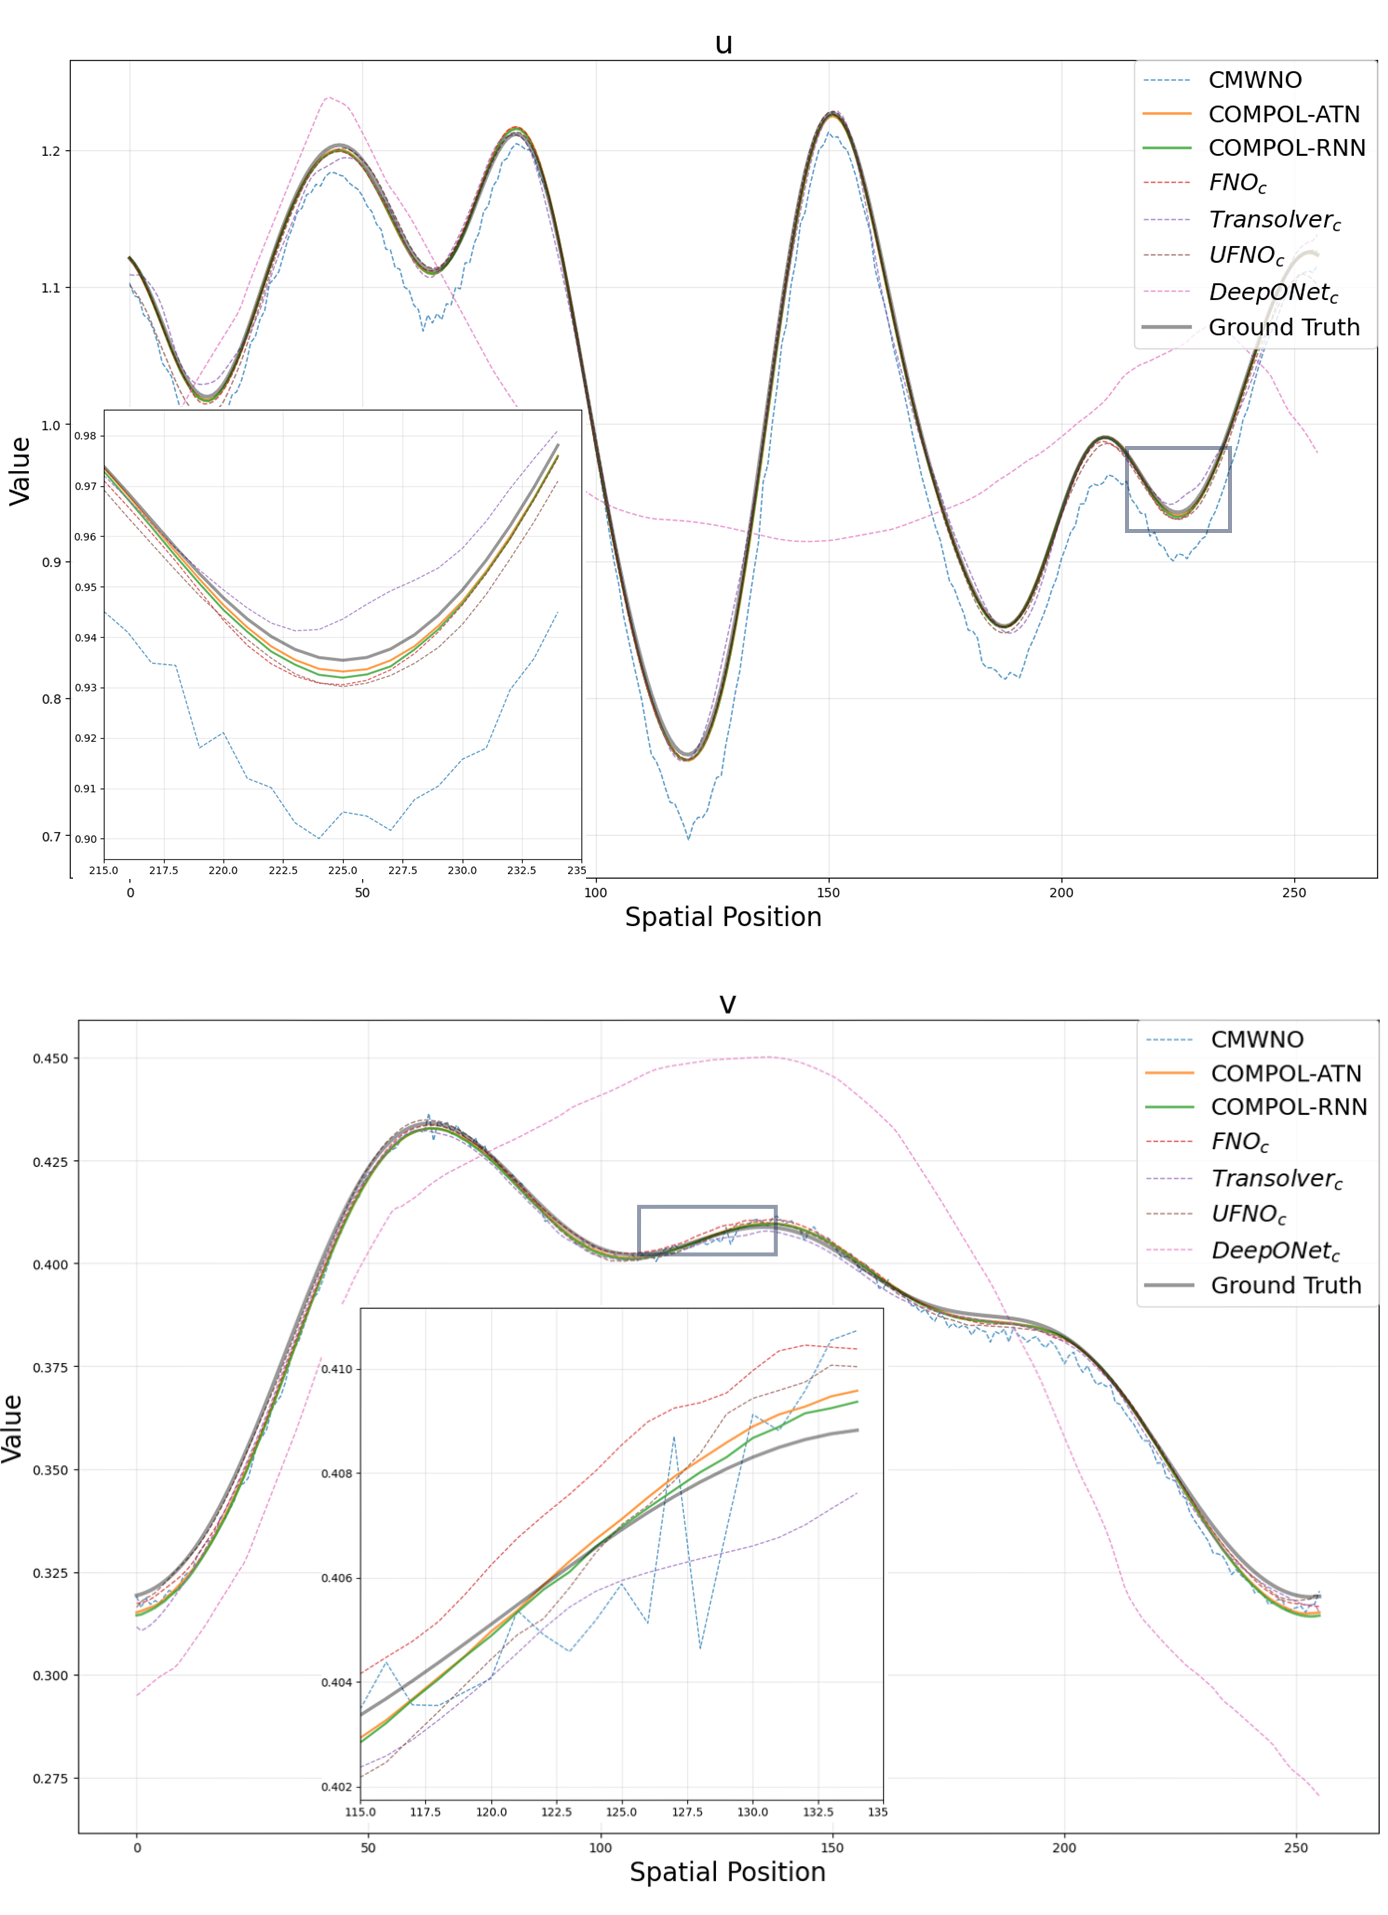
\includegraphics[width=1.0\textwidth]{figs/pred_ground/LV_plots_vertical.png}
	\caption{
		Predictions of \ours and Baseline Models vs. Ground Truth of Lotka-Volterra Using 512 Training Samples
	}
	\label{fig:LV_512_pred_ground}
\end{figure*}

\begin{figure*}[!htbp]
	\centering
	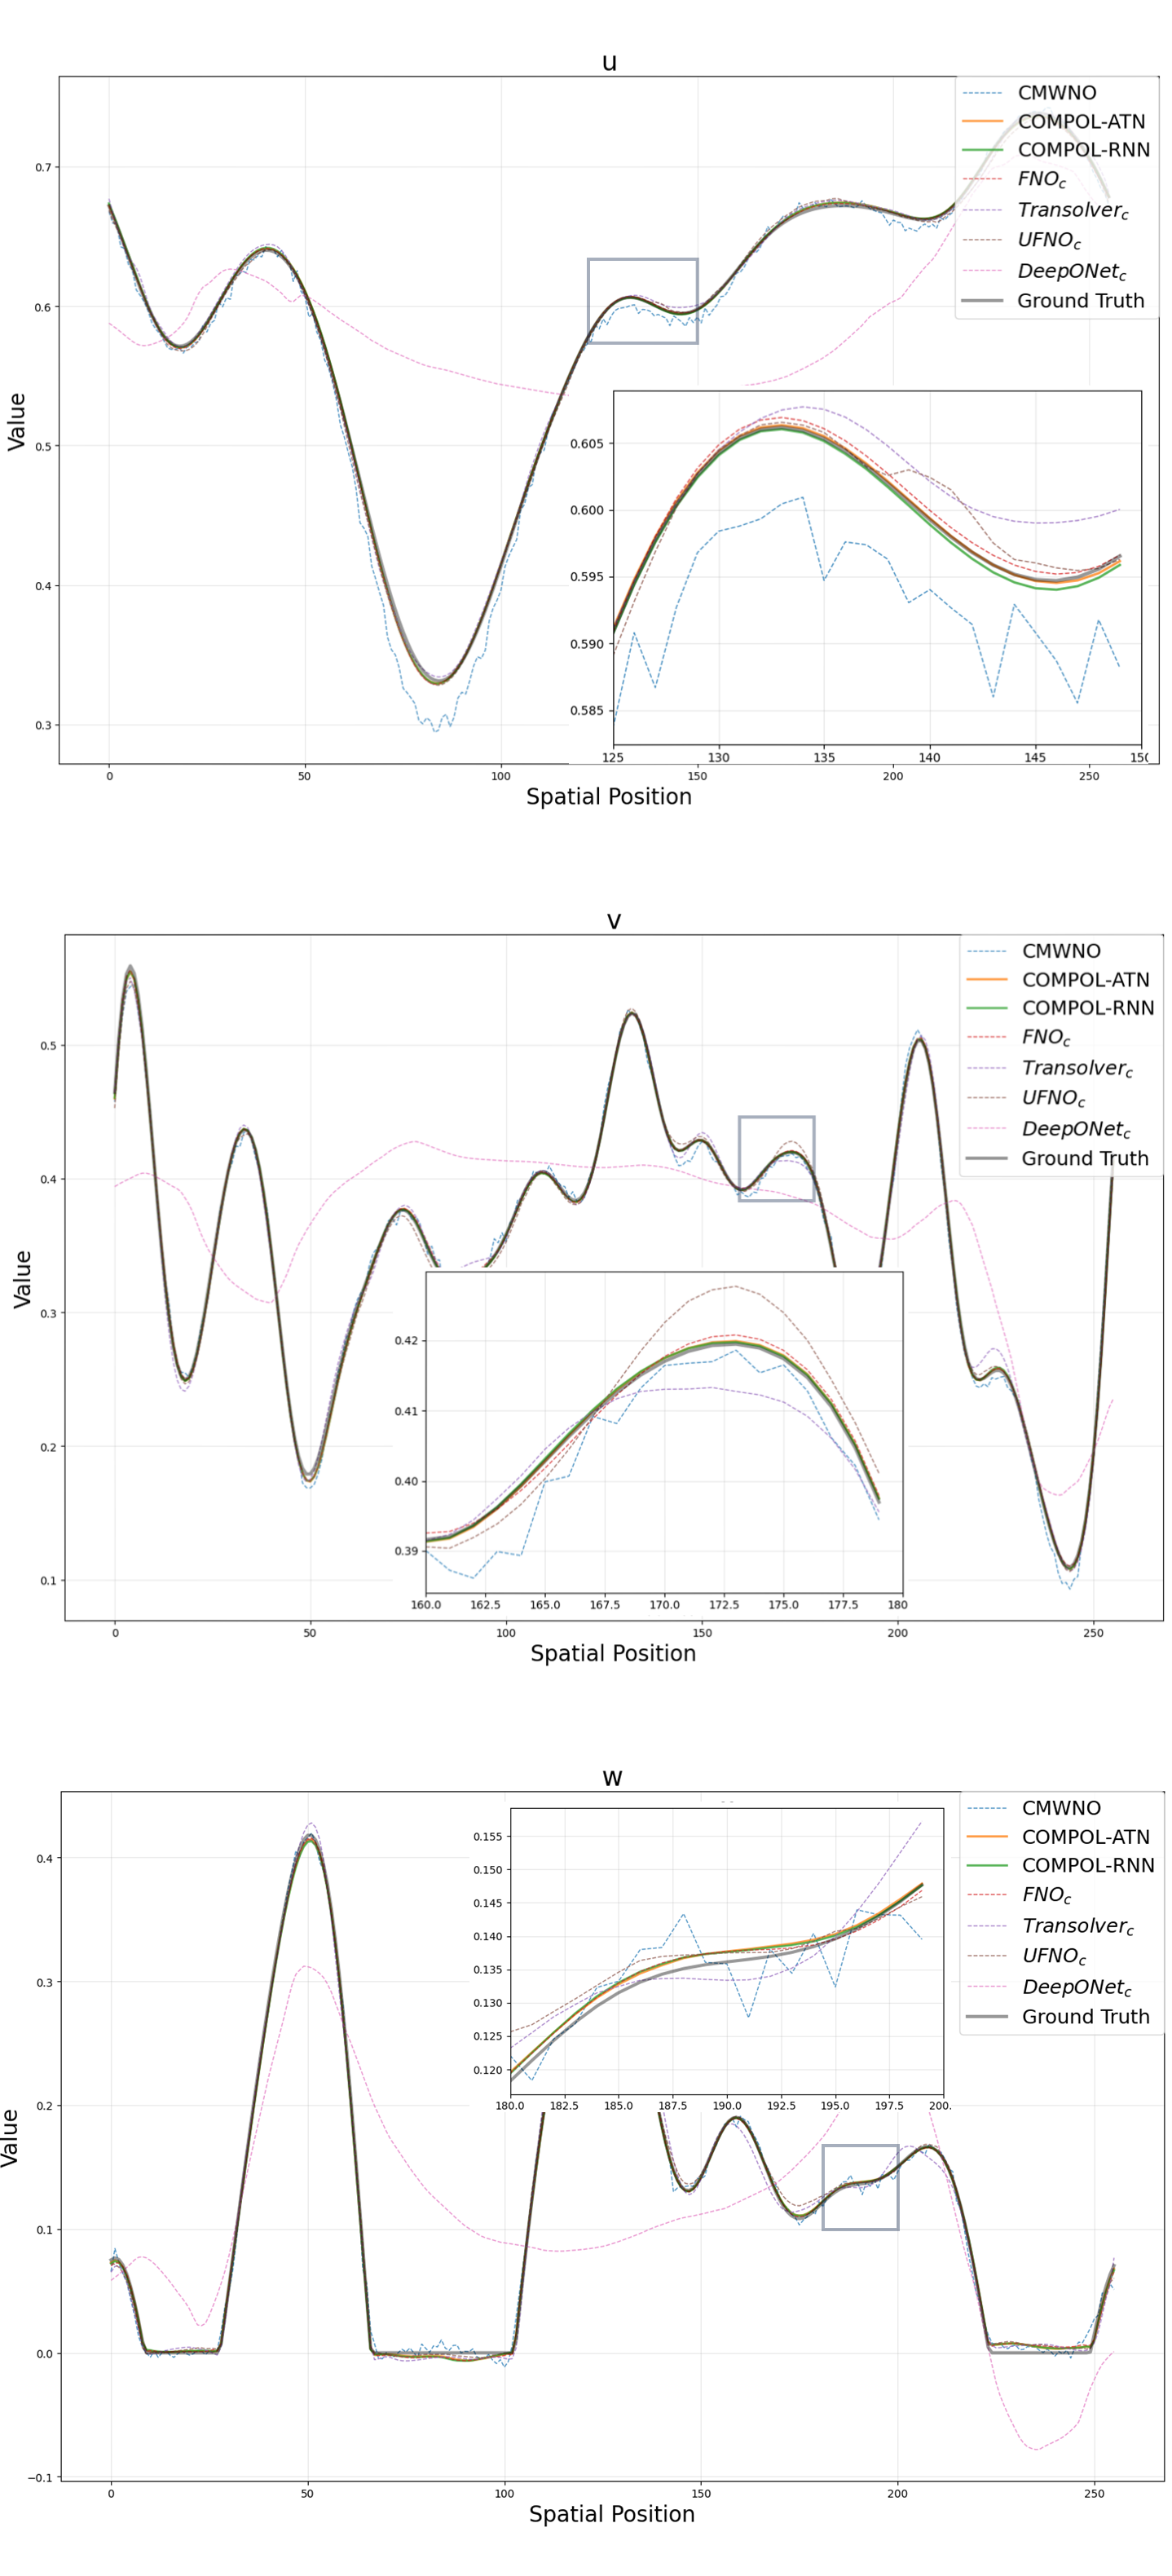
\includegraphics[width=0.7\textwidth]{figs/pred_ground/BZ_plots_vertical.png}
	\caption{
		Predictions of \ours and Baseline Models vs. Ground Truth of Belousov-Zhabotinsky Using 512 Training Samples
	}
	\label{fig:BZ_512_pred_ground}
\end{figure*}


\newpage
\section{A Comprehensive Investigation of \ours's Coupling Mechanisms}
\label{sec:appx-coupling}

According to Figure \ref{fig:model}, our proposed model consists of three key components: (1) $c_{l-1}$ compresses and aggregates outputs from multiple processes, denoted as $\mathbf{v}_{l-1}^p\ (p=1,...,M)$, at the current layer; (2) $a_{l-1}$ aggregates latent representations from all previous layers, $\mathcal{V}_{l-1}$; and (3) $b_{l-1}$ integrates the aggregated information back into the original process-specific outputs $\mathbf{v}_{l-1}^p$. The default implementations for these components are linear transformation for $c_{l-1}$, attention mechanisms for $a_{l-1}$, and simple addition for $b_{l-1}$. Alternative configurations tested include: replacing linear transformation in $c_{l-1}$ with addition; substituting the attention mechanism in $a_{l-1}$ with ResNet-style skip connections, RNN, or multihead attention; and using concatenation followed by dimensionality reduction instead of addition for $b_{l-1}$. We particularly examined alternative methods for $a_{l-1}$ to explore how attention compares against less expressive methods like RNNs or ResNet-like skip connections, which inherently discard older information from layers further back.

We also explored the impact of employing separate Fourier Neural Operators (FNOs) for each process versus a single FNO treating all processes as channels. Additionally, we varied the model width parameter to investigate how performance scales with the number of parameters, limited to one-dimensional cases due to computational constraints.

Figures \ref{fig:LV_512_fnoperc_vs_testerr} to \ref{fig:LV_512_params_vs_testtrainratio} summarize performance evaluations of 160 models. Dot labels indicate the width parameter, with negative values representing fewer parameters and positive values indicating increased parameters. Standard deviations are shown by error bars. Figure \ref{fig:LV_512_fnoperc_vs_testerr} reveals a general trend where separate FNOs with linear transformation outperform those with additive mixing, single FNO models, and separate FNOs without inter-process communication. Test error versus parameter percentage demonstrates a U-shaped curve, with optimal performance around 90\%. In Figure \ref{fig:LV_512_params_vs_testerr}, attention and RNN aggregation significantly decrease test errors in separate FNO scenarios but adversely impact performance in single FNO setups. Our model consistently achieves superior results across various parameter settings, particularly with attention mechanisms. Differences between additive and concatenative approaches in $b_{l-1}$ are minimal. Figure \ref{fig:LV_512_params_vs_trainerr} shows a clear scaling law, as logarithmic training errors decrease linearly with logarithmic parameter increases. Figure \ref{fig:LV_512_params_vs_testtrainratio} indicates that overfitting occurs as parameter counts become large. Notably, separate FNOs without inter-process communication perform poorly, emphasizing the critical role of effective information mixing.

Similar trends are evident in results from the Belousov-Zhabotinsky equations (Figures \ref{fig:BZ_512_fnoperc_vs_testerr}–\ref{fig:BZ_512_params_vs_testtrainratio}). Additionally, Figure \ref{fig:Burgers_512_params_vs_testerr} demonstrates that even for single-process scenarios like the 1D Burgers equation, our model's ResNet-like architecture significantly enhances performance by enabling deeper layers to learn residual corrections rather than entire solutions.

We further evaluated model performance on deliberately unrelated processes by concatenating distinct channels from Belousov-Zhabotinsky, Lotka-Volterra, and Burgers equations. Figures \ref{fig:synthetic_512_FNOperc_vs_testerr} and \ref{fig:synthetic_512_params_vs_testerr} indicate that standard FNOs perform poorly in this setting due to inefficient interchannel communication in the frequency domain. In contrast, our model, based on separate FNOs with controlled inter-process communication in the spatial-temporal domain, performs robustly, matching or slightly surpassing separate FNO performance. This advantage highlights our model's capability to flexibly manage both strongly and weakly related processes without requiring prior knowledge of their interplay, making it highly suitable for fully data-driven scenarios.

In conclusion, the ablation study consistently demonstrates that our proposed architecture outperforms alternative configurations under equivalent parameter budgets. Modifying or omitting components generally leads to performance degradation, underscoring the effectiveness of the integrated design.


\begin{figure*}[!htbp]
	\centering
	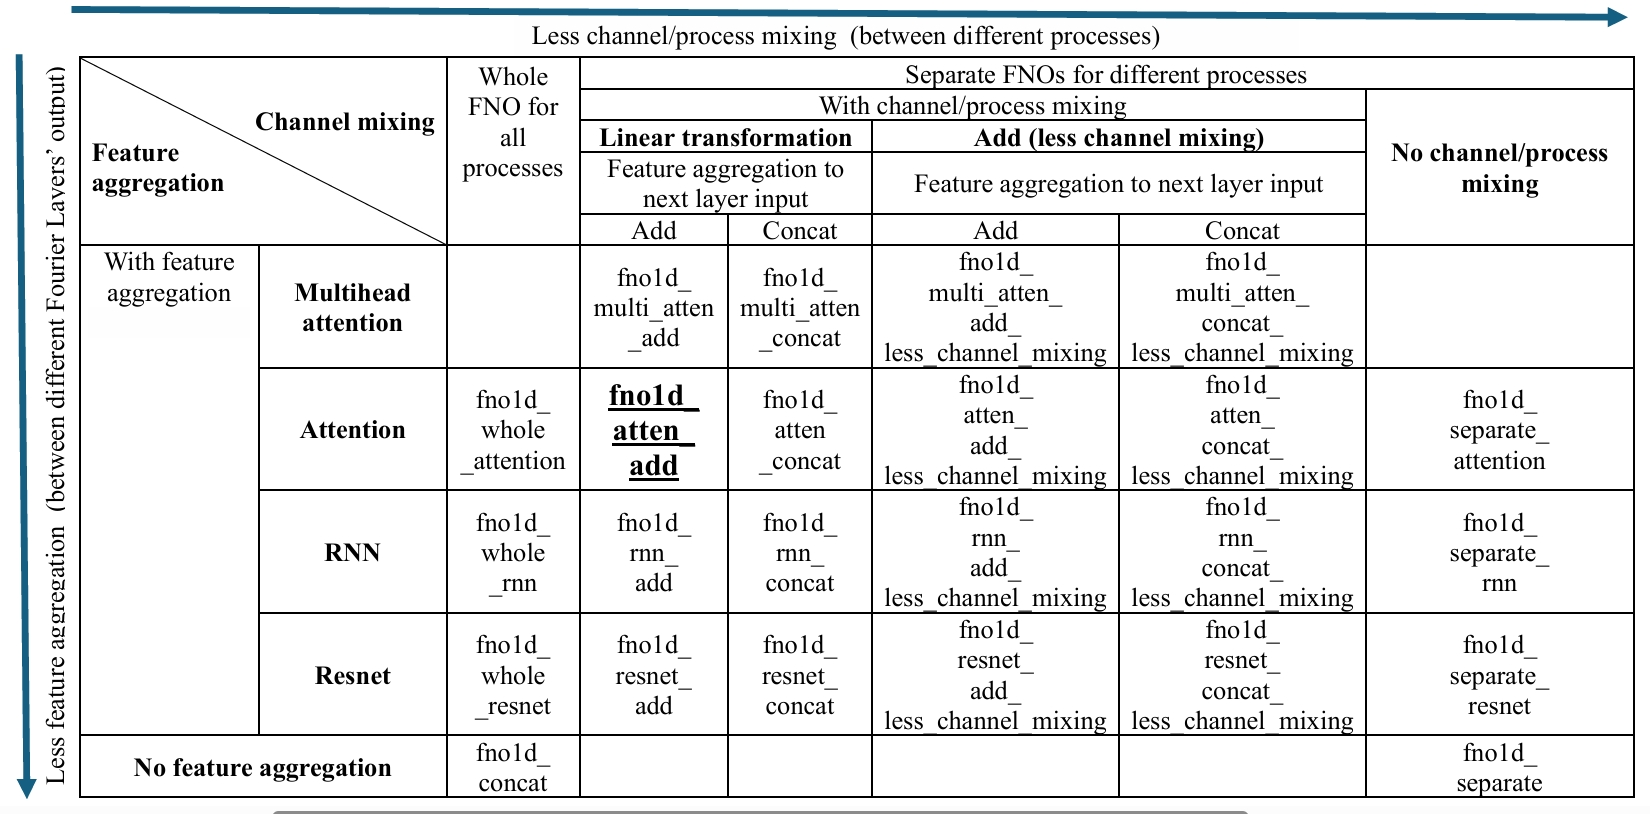
\includegraphics[width=1.0\textwidth]{figs/ablation.png}
	\caption{
		Models tested in the ablation study arranged by two dimensions: feature aggregation of layers and channel/process mixing. fno1d\_atten\_add is the model we use by default
	}
	\label{fig:ablation}
\end{figure*}


\begin{figure*}[!htbp]
	\centering
	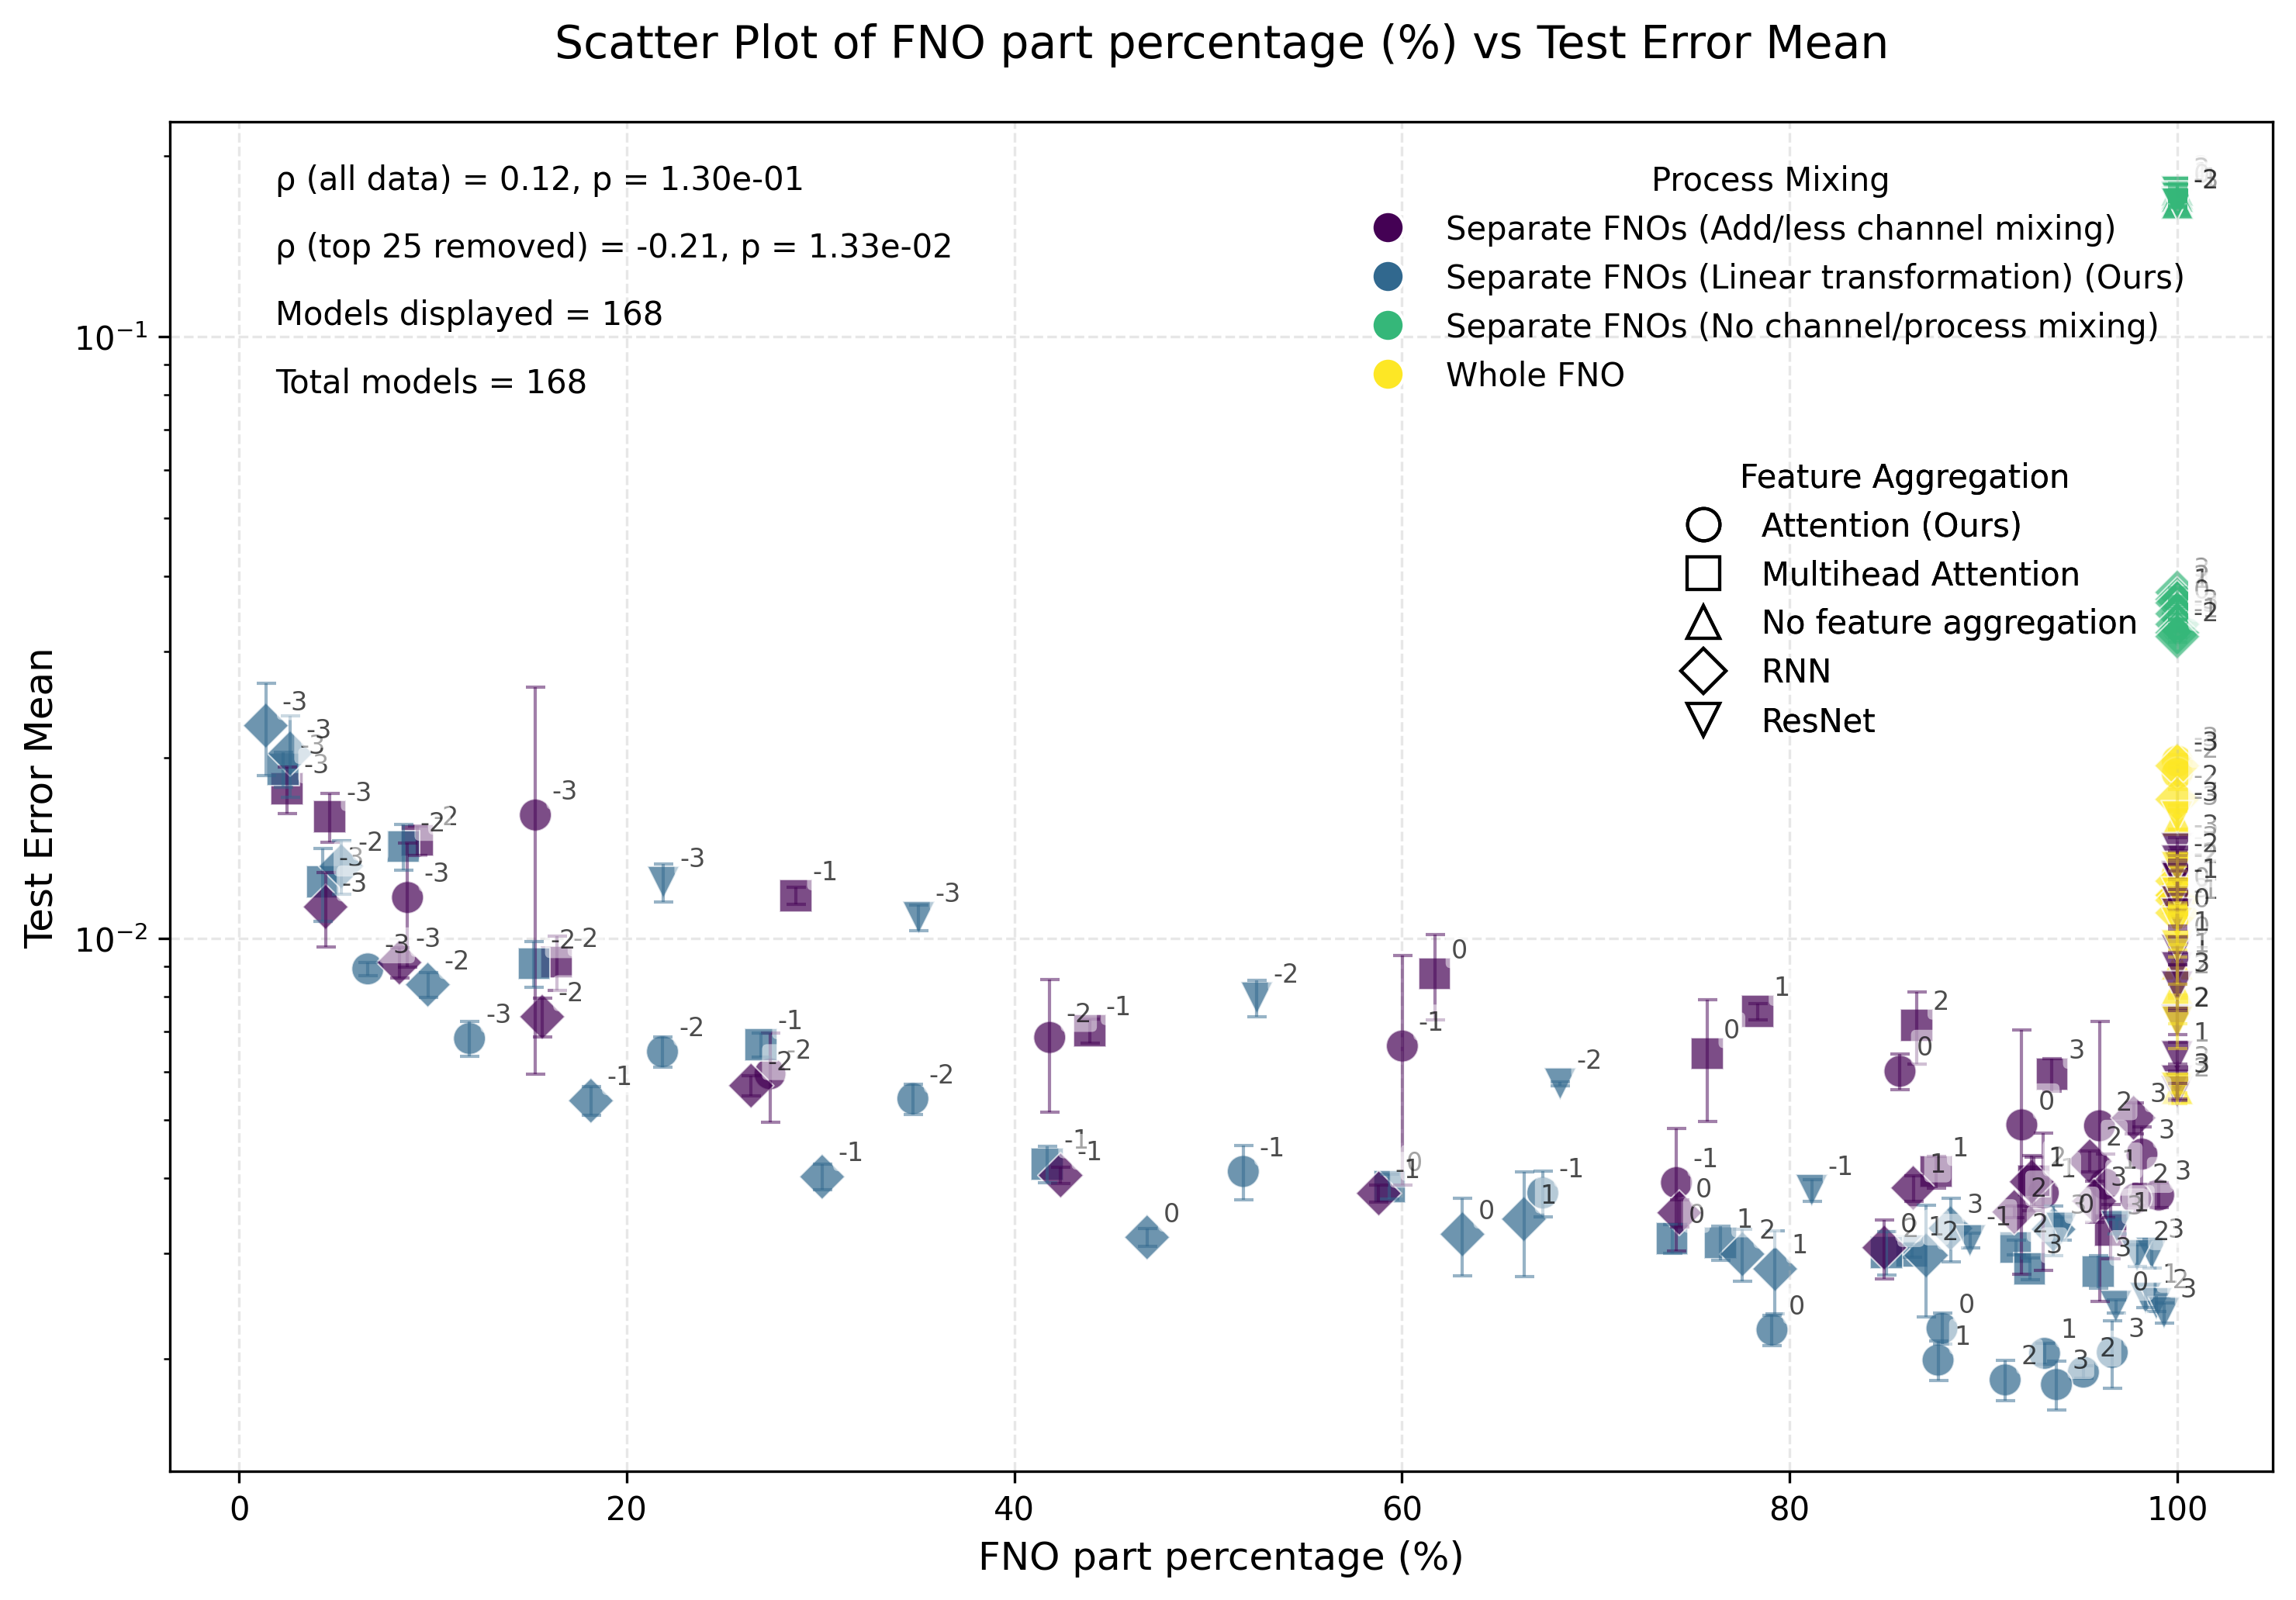
\includegraphics[width=1.0\textwidth]{figs/ablation_figs/LV_512_fnoperc_vs_testerr.png}
	\caption{
		Test Errors vs Percentage of FNO Parameters of Lotka-Volterra Using 512 Training Samples
	}
	\label{fig:LV_512_fnoperc_vs_testerr}
\end{figure*}

\begin{figure*}[!htbp]
	\centering
	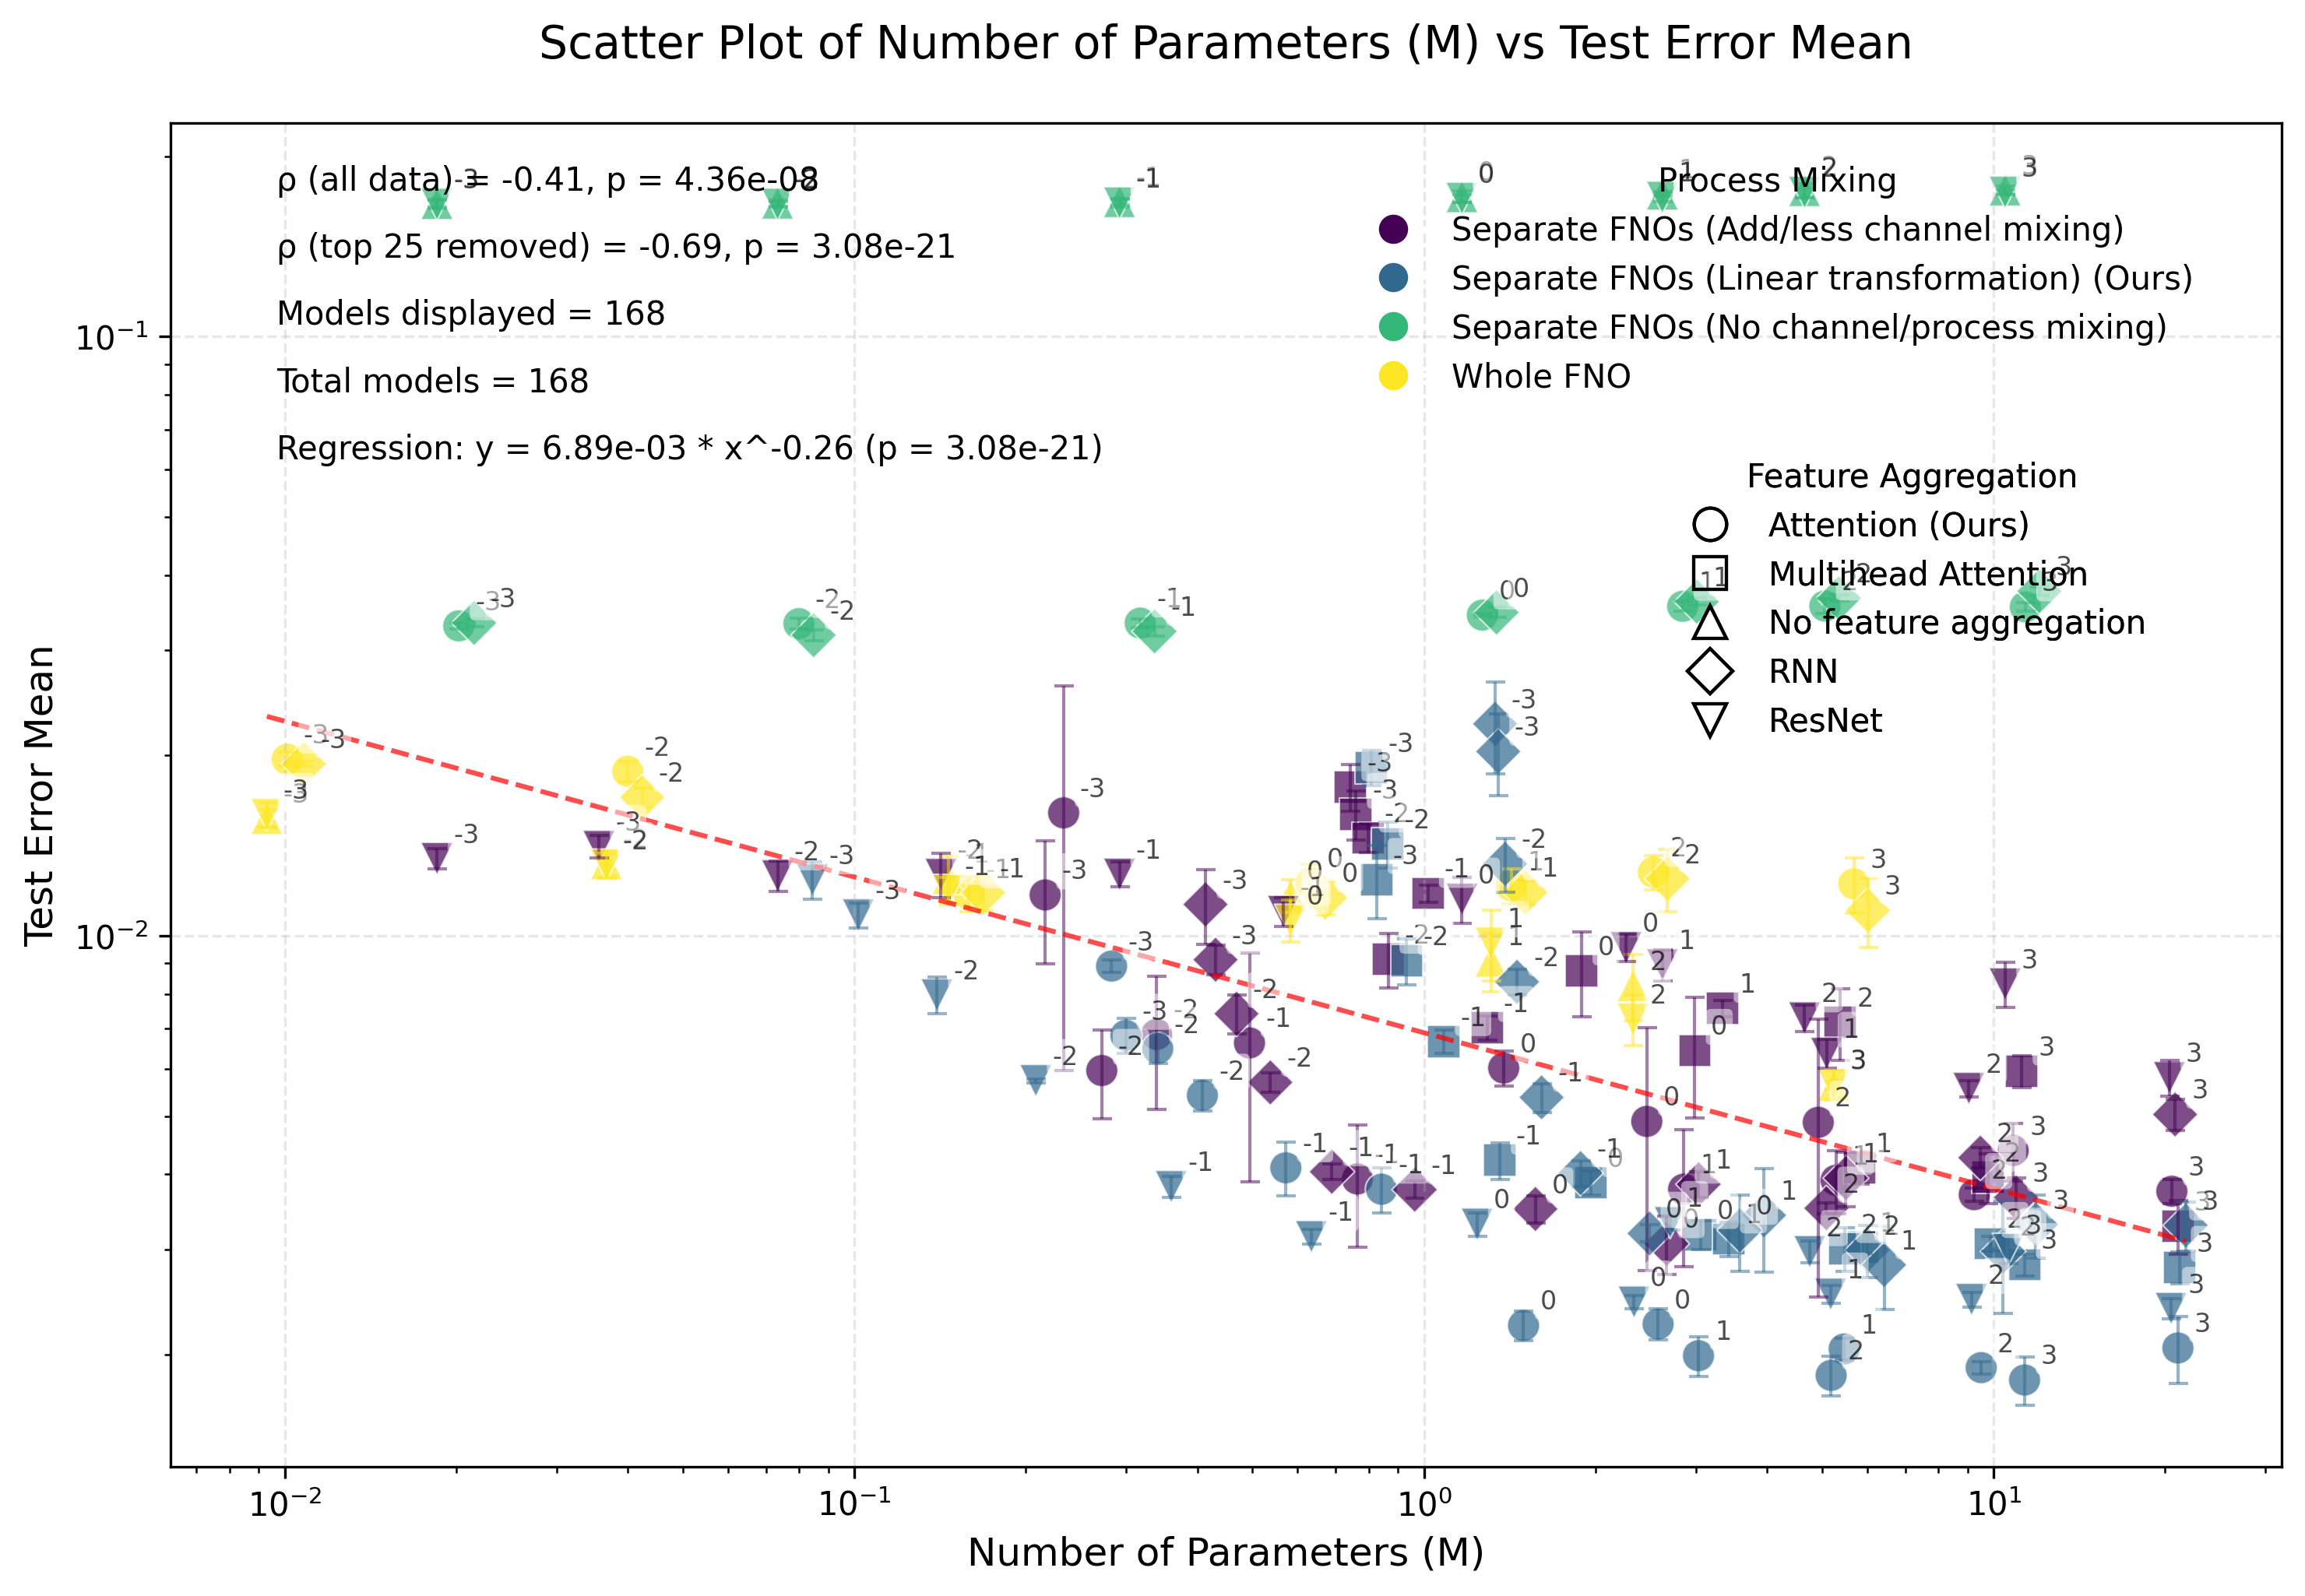
\includegraphics[width=1.0\textwidth]{figs/ablation_figs/LV_512_params_vs_testerr.png}
	\caption{
		Test Errors vs Number of Parameters of Lotka-Volterra Using 512 Training Samples
	}
	\label{fig:LV_512_params_vs_testerr}
\end{figure*}

\begin{figure*}[!htbp]
	\centering
	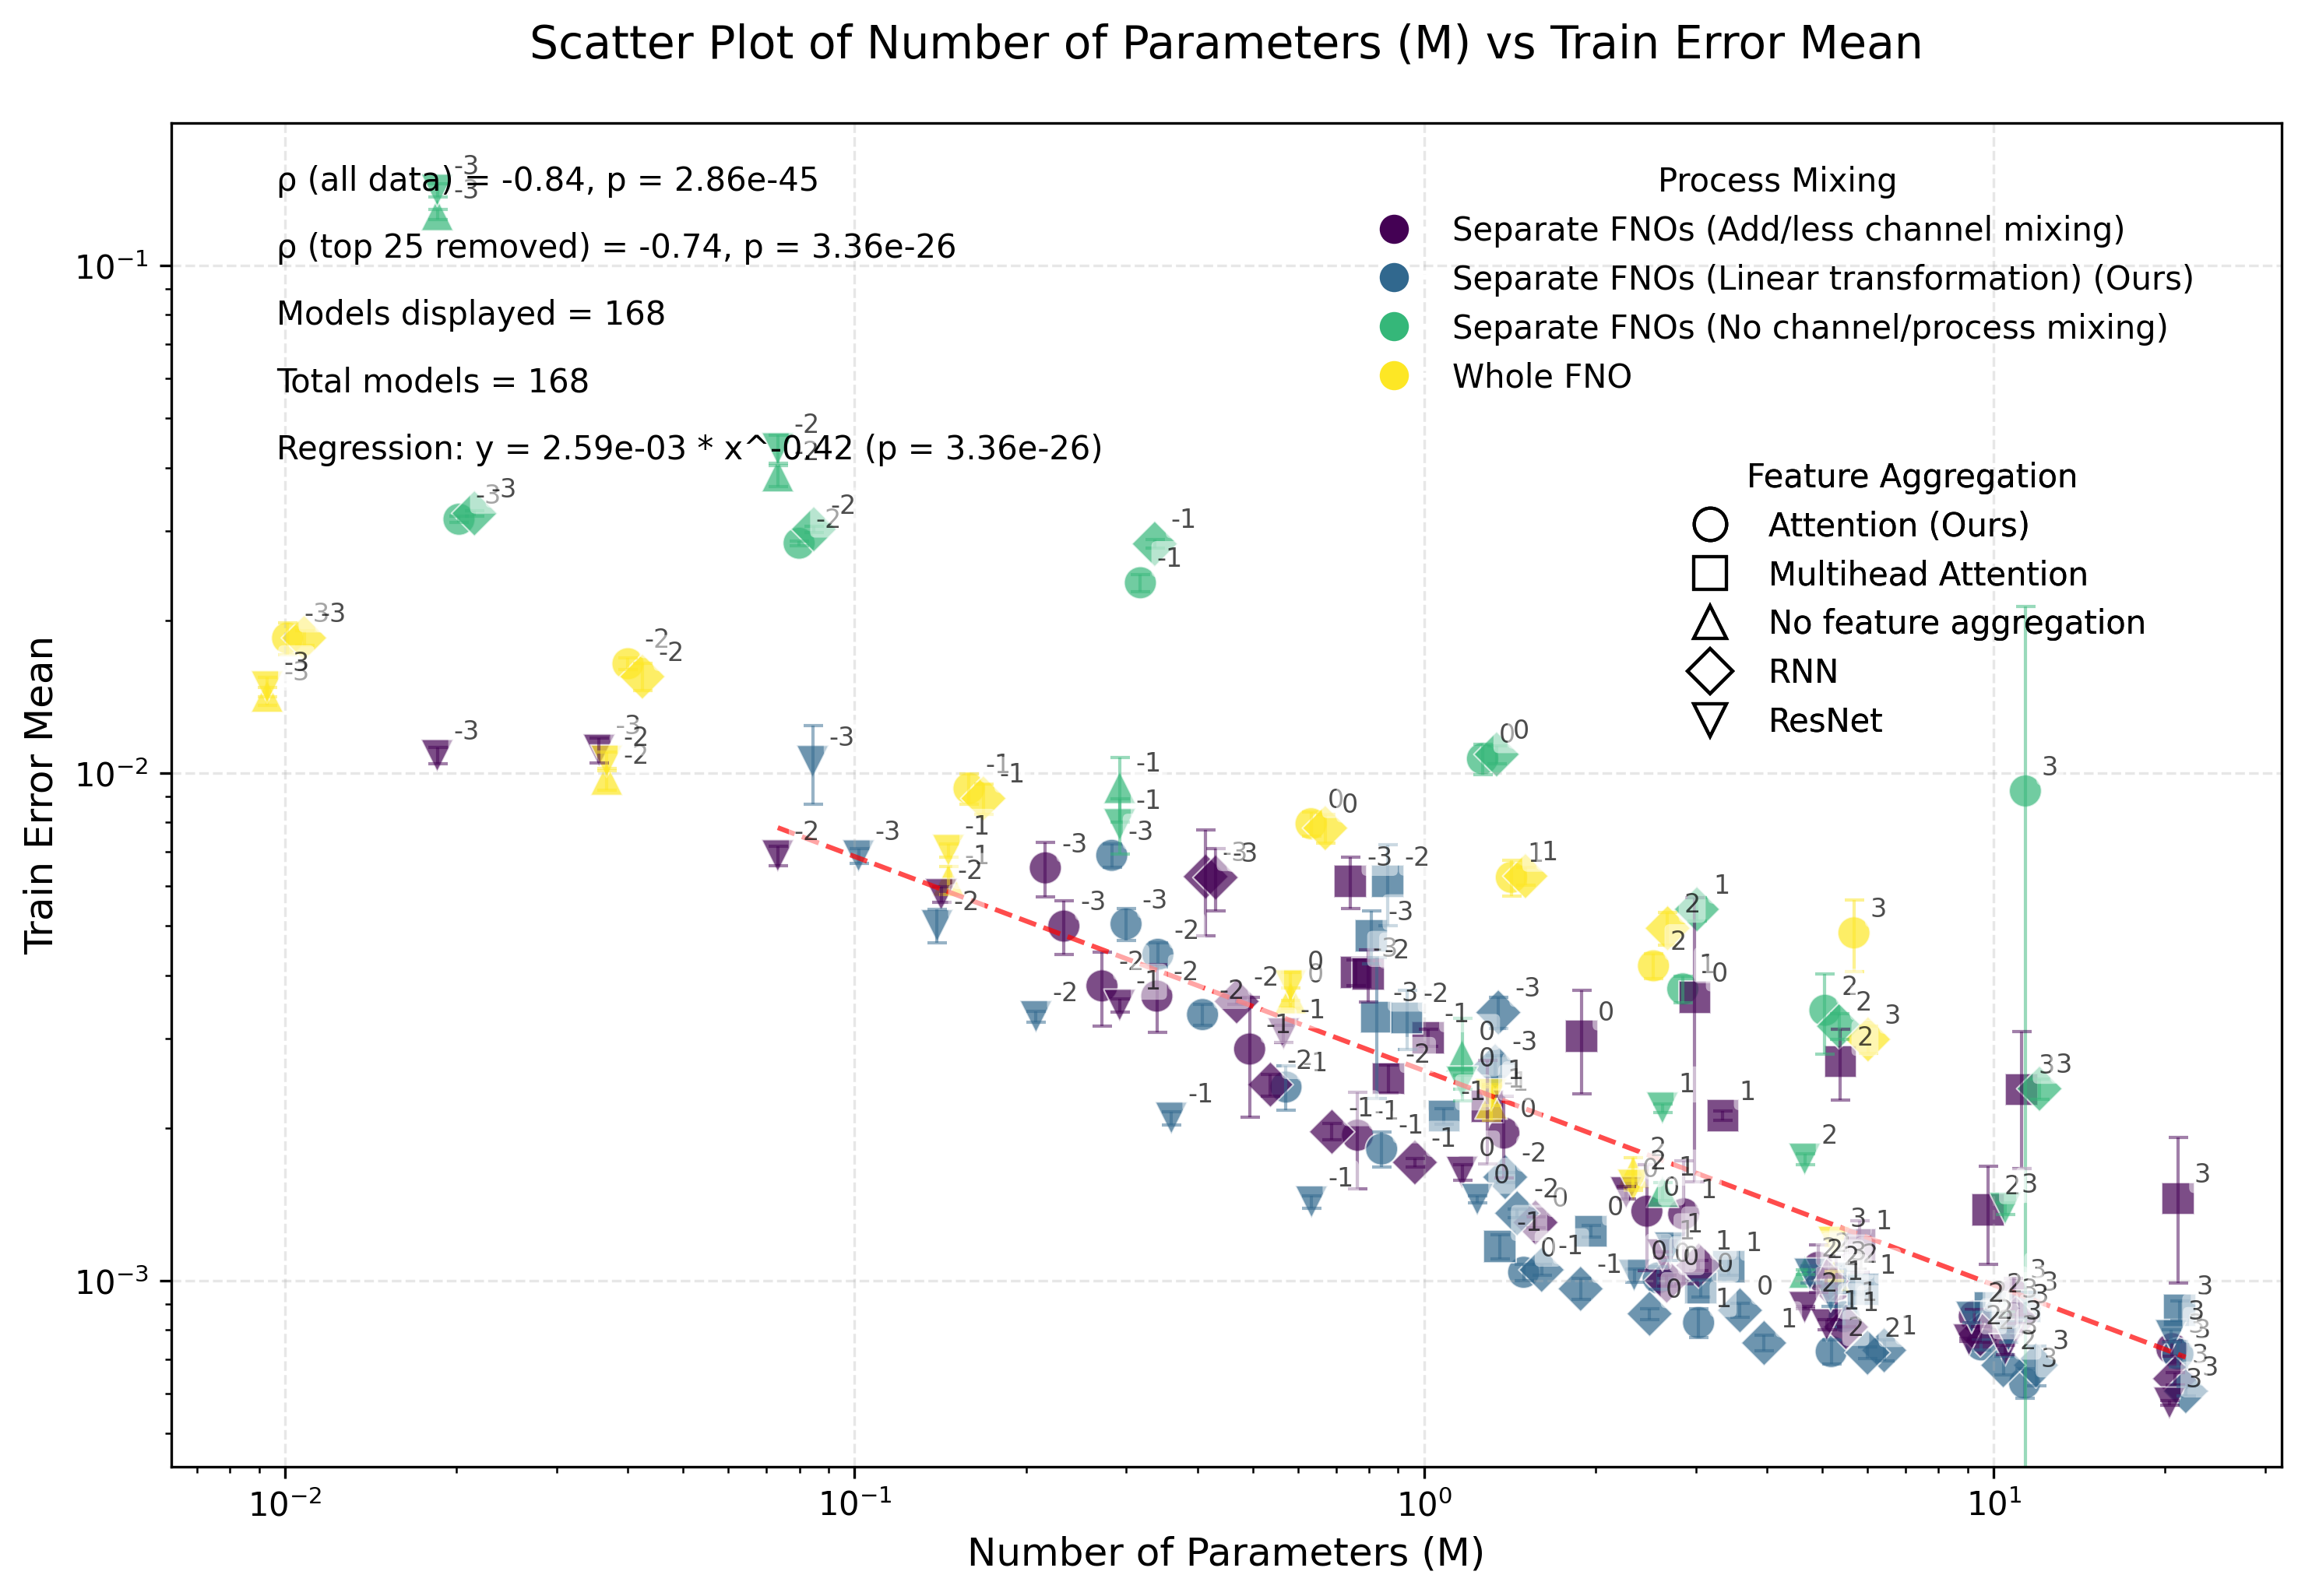
\includegraphics[width=1.0\textwidth]{figs/ablation_figs/LV_512_params_vs_trainerr.png}
	\caption{
		Test Errors vs Number of Parameters of Lotka-Volterra Using 512 Training Samples
	}
	\label{fig:LV_512_params_vs_trainerr}
\end{figure*}

\begin{figure*}[!htbp]
	\centering
	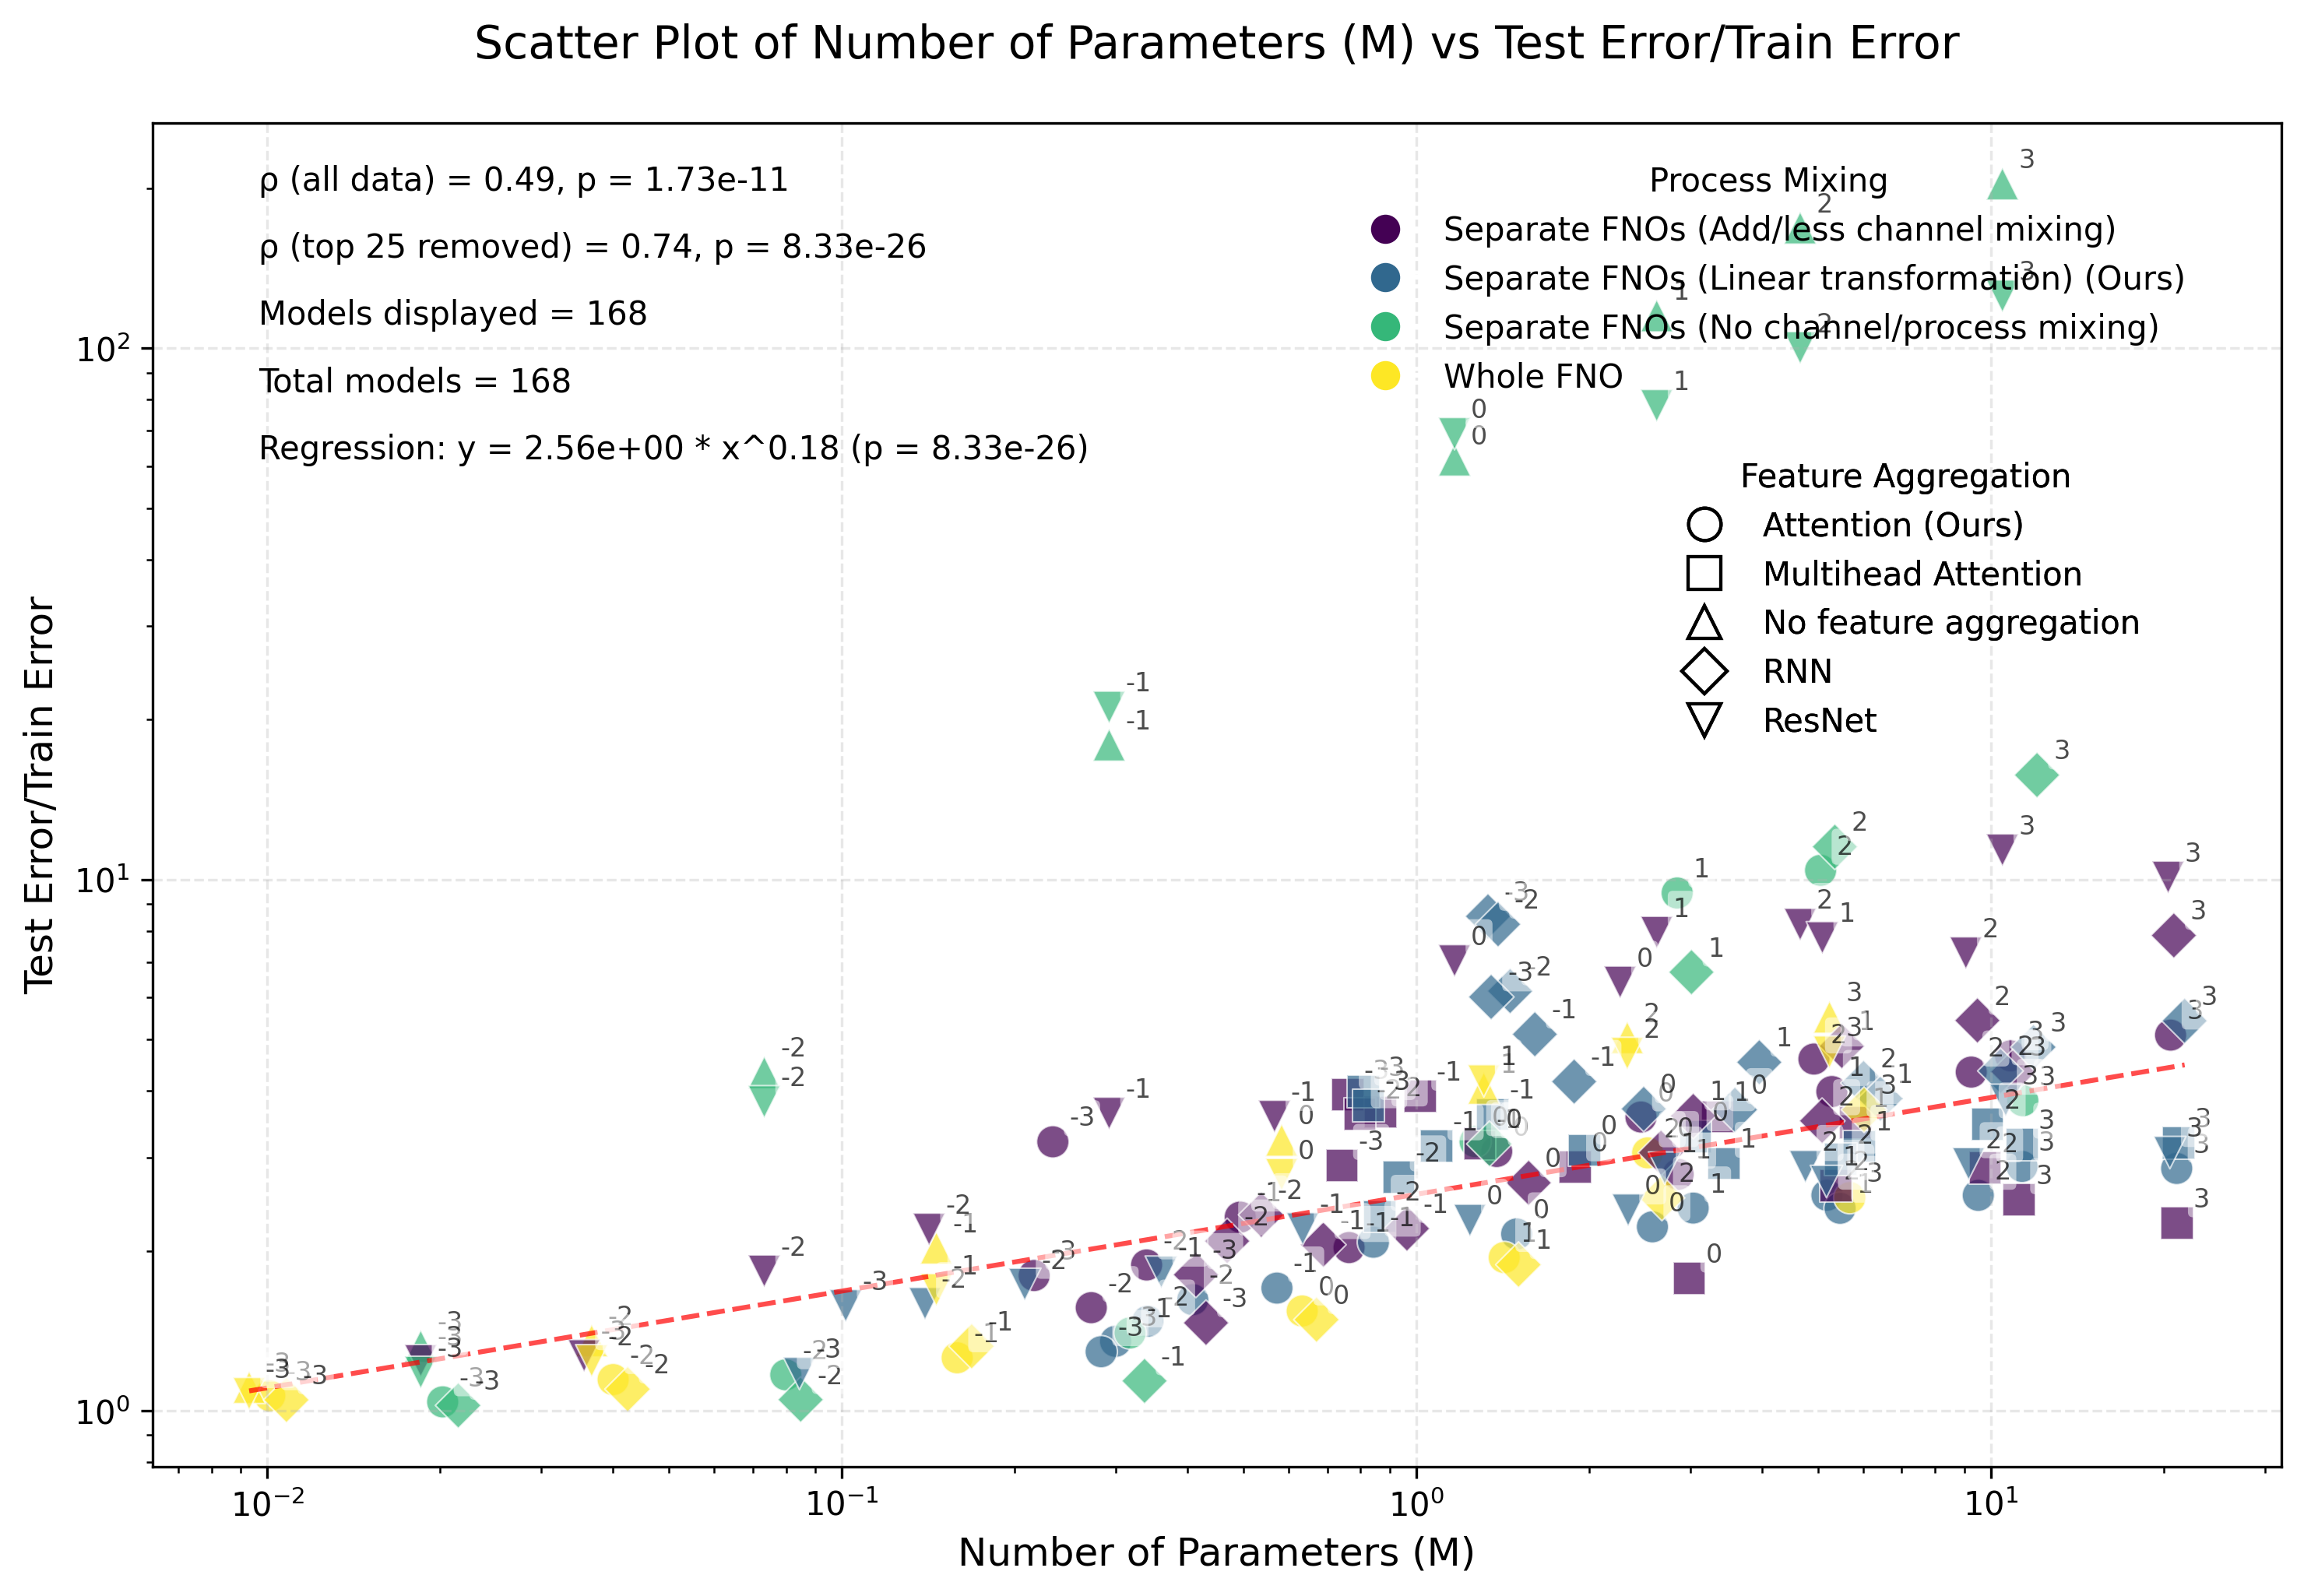
\includegraphics[width=1.0\textwidth]{figs/ablation_figs/LV_512_params_vs_testtrainratio.png}
	\caption{
		Test Errors Over Train Errors Ratio vs Number of Parameters of Lotka-Volterra Using 512 Training Samples
	}
	\label{fig:LV_512_params_vs_testtrainratio}
\end{figure*}

\begin{figure*}[!htbp]
	\centering
	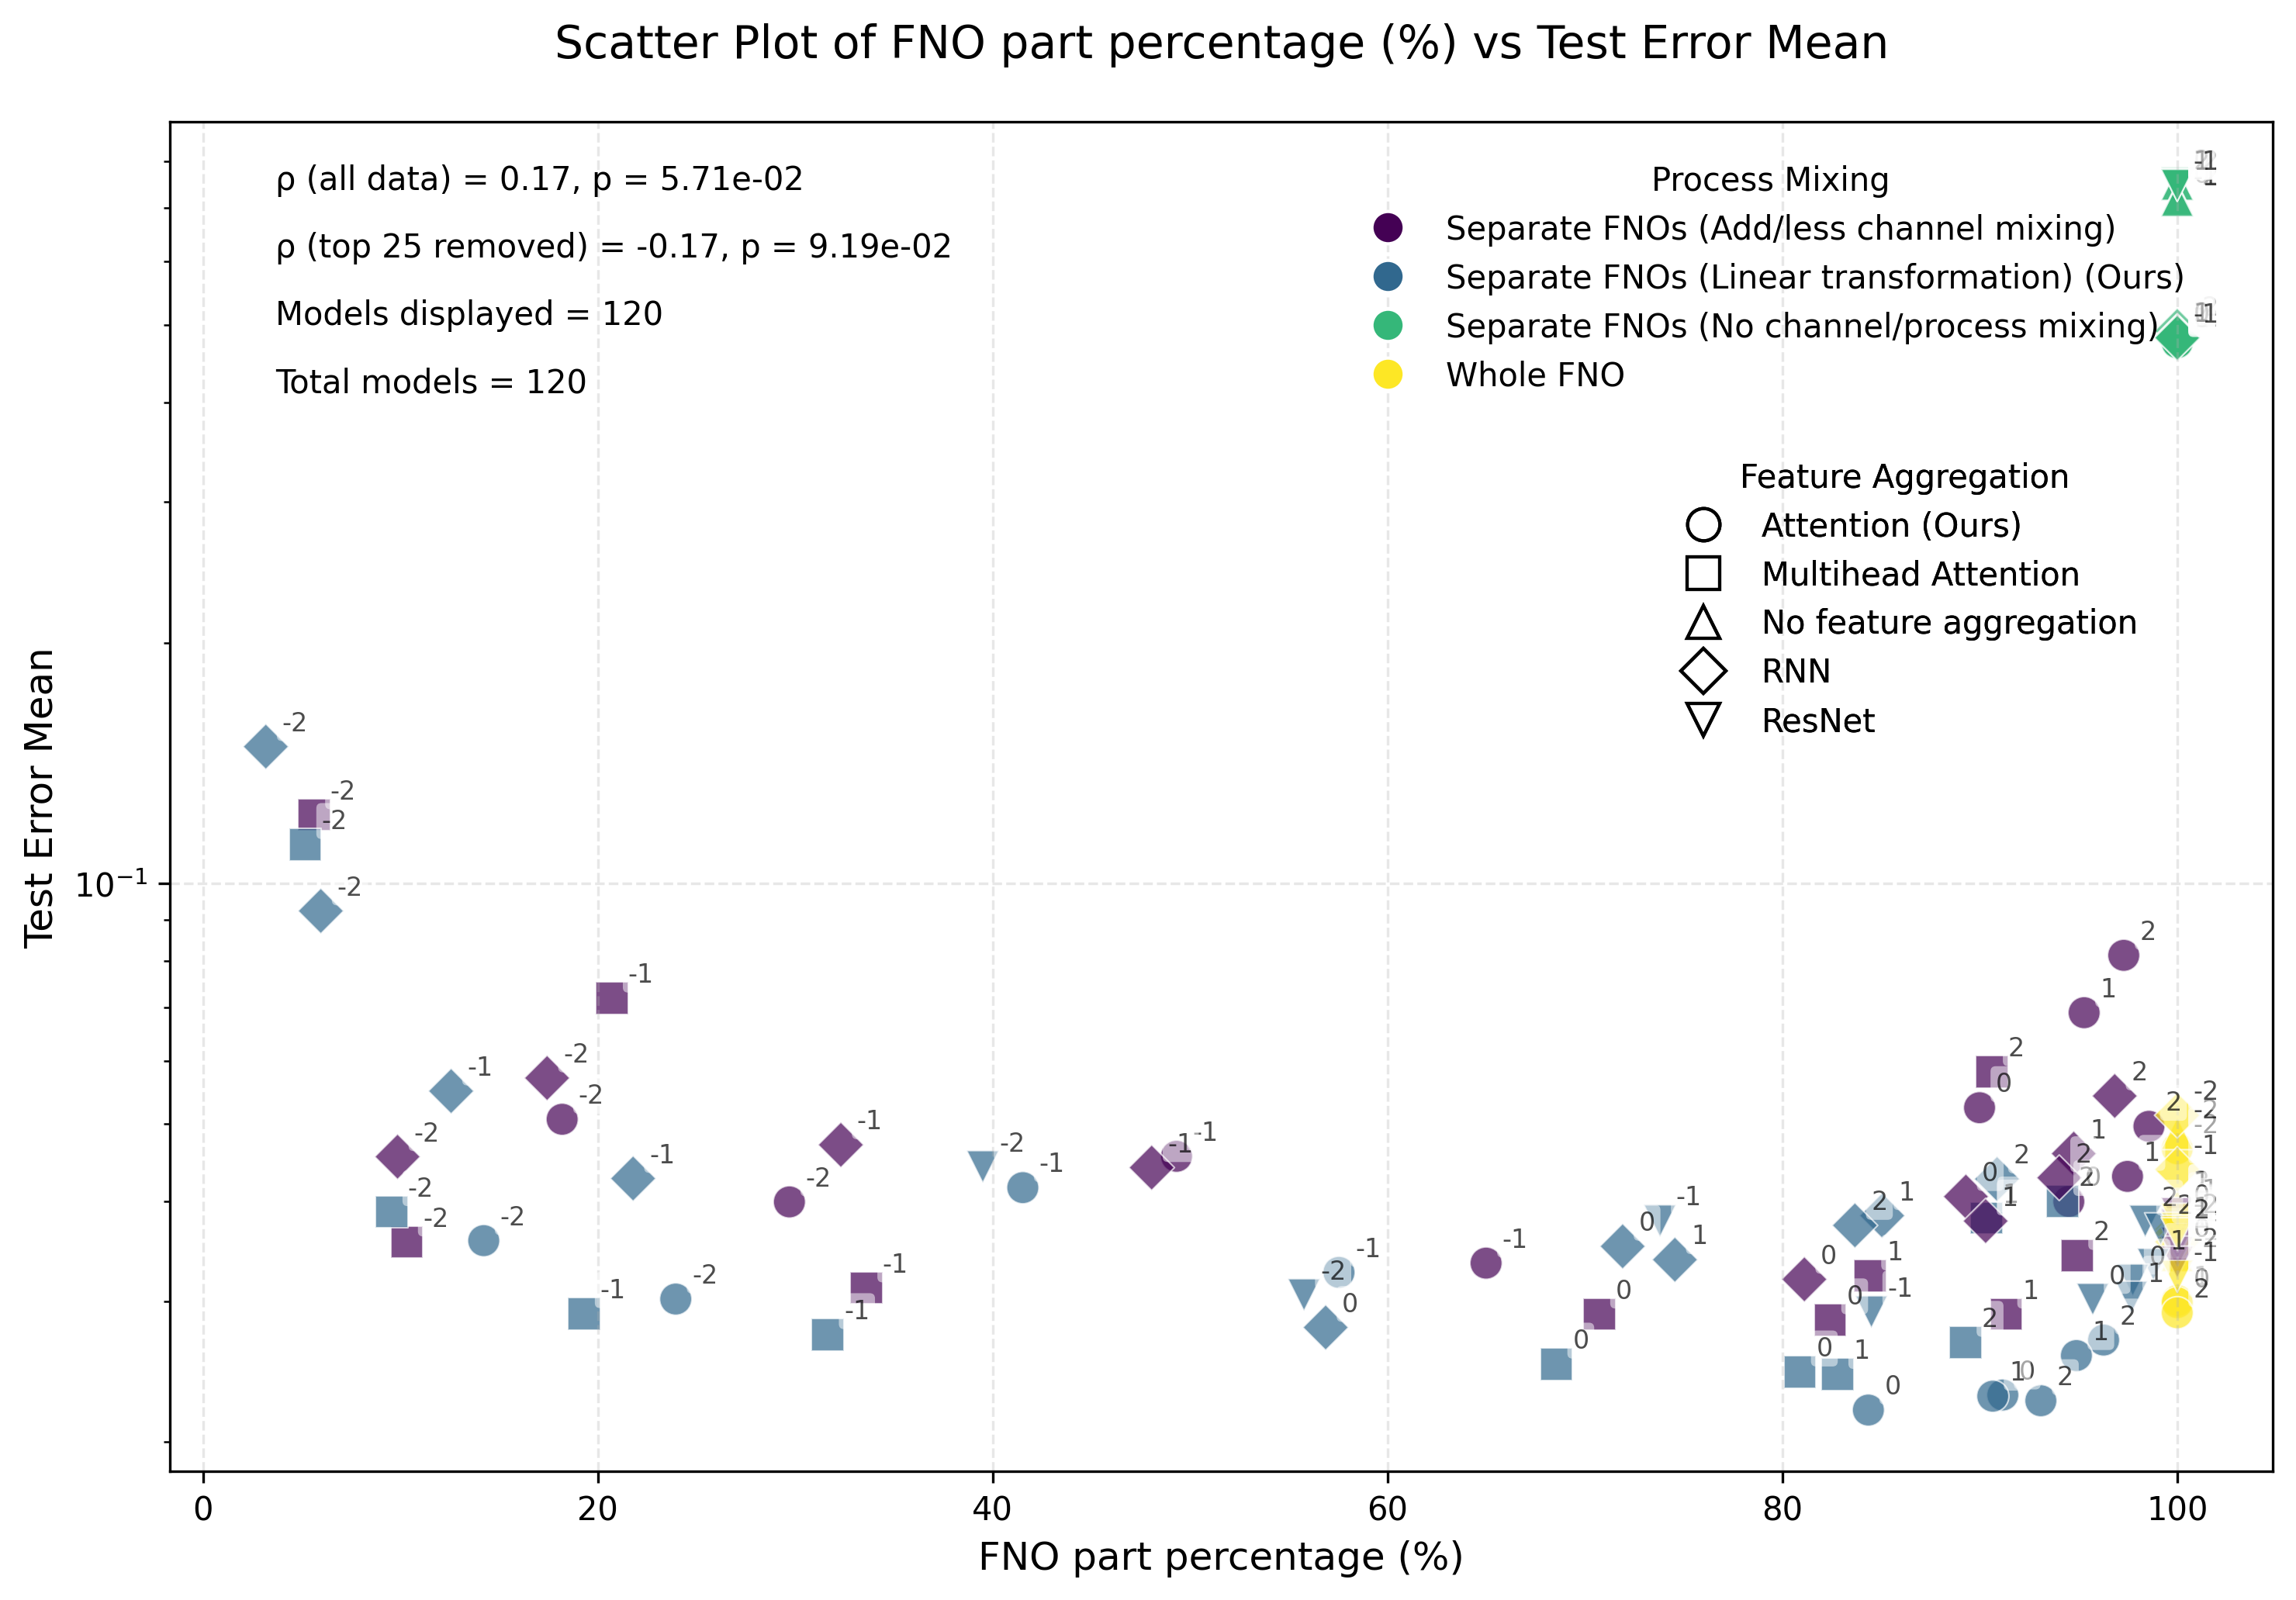
\includegraphics[width=1.0\textwidth]{figs/ablation_figs/BZ_512_fnoperc_vs_testerr.png}
	\caption{
		Test Errors vs Percentage of FNO Parameters of Belousov-Zhabotinsky Using 512 Training Samples
	}
	\label{fig:BZ_512_fnoperc_vs_testerr}
\end{figure*}

\begin{figure*}[!htbp]
	\centering
	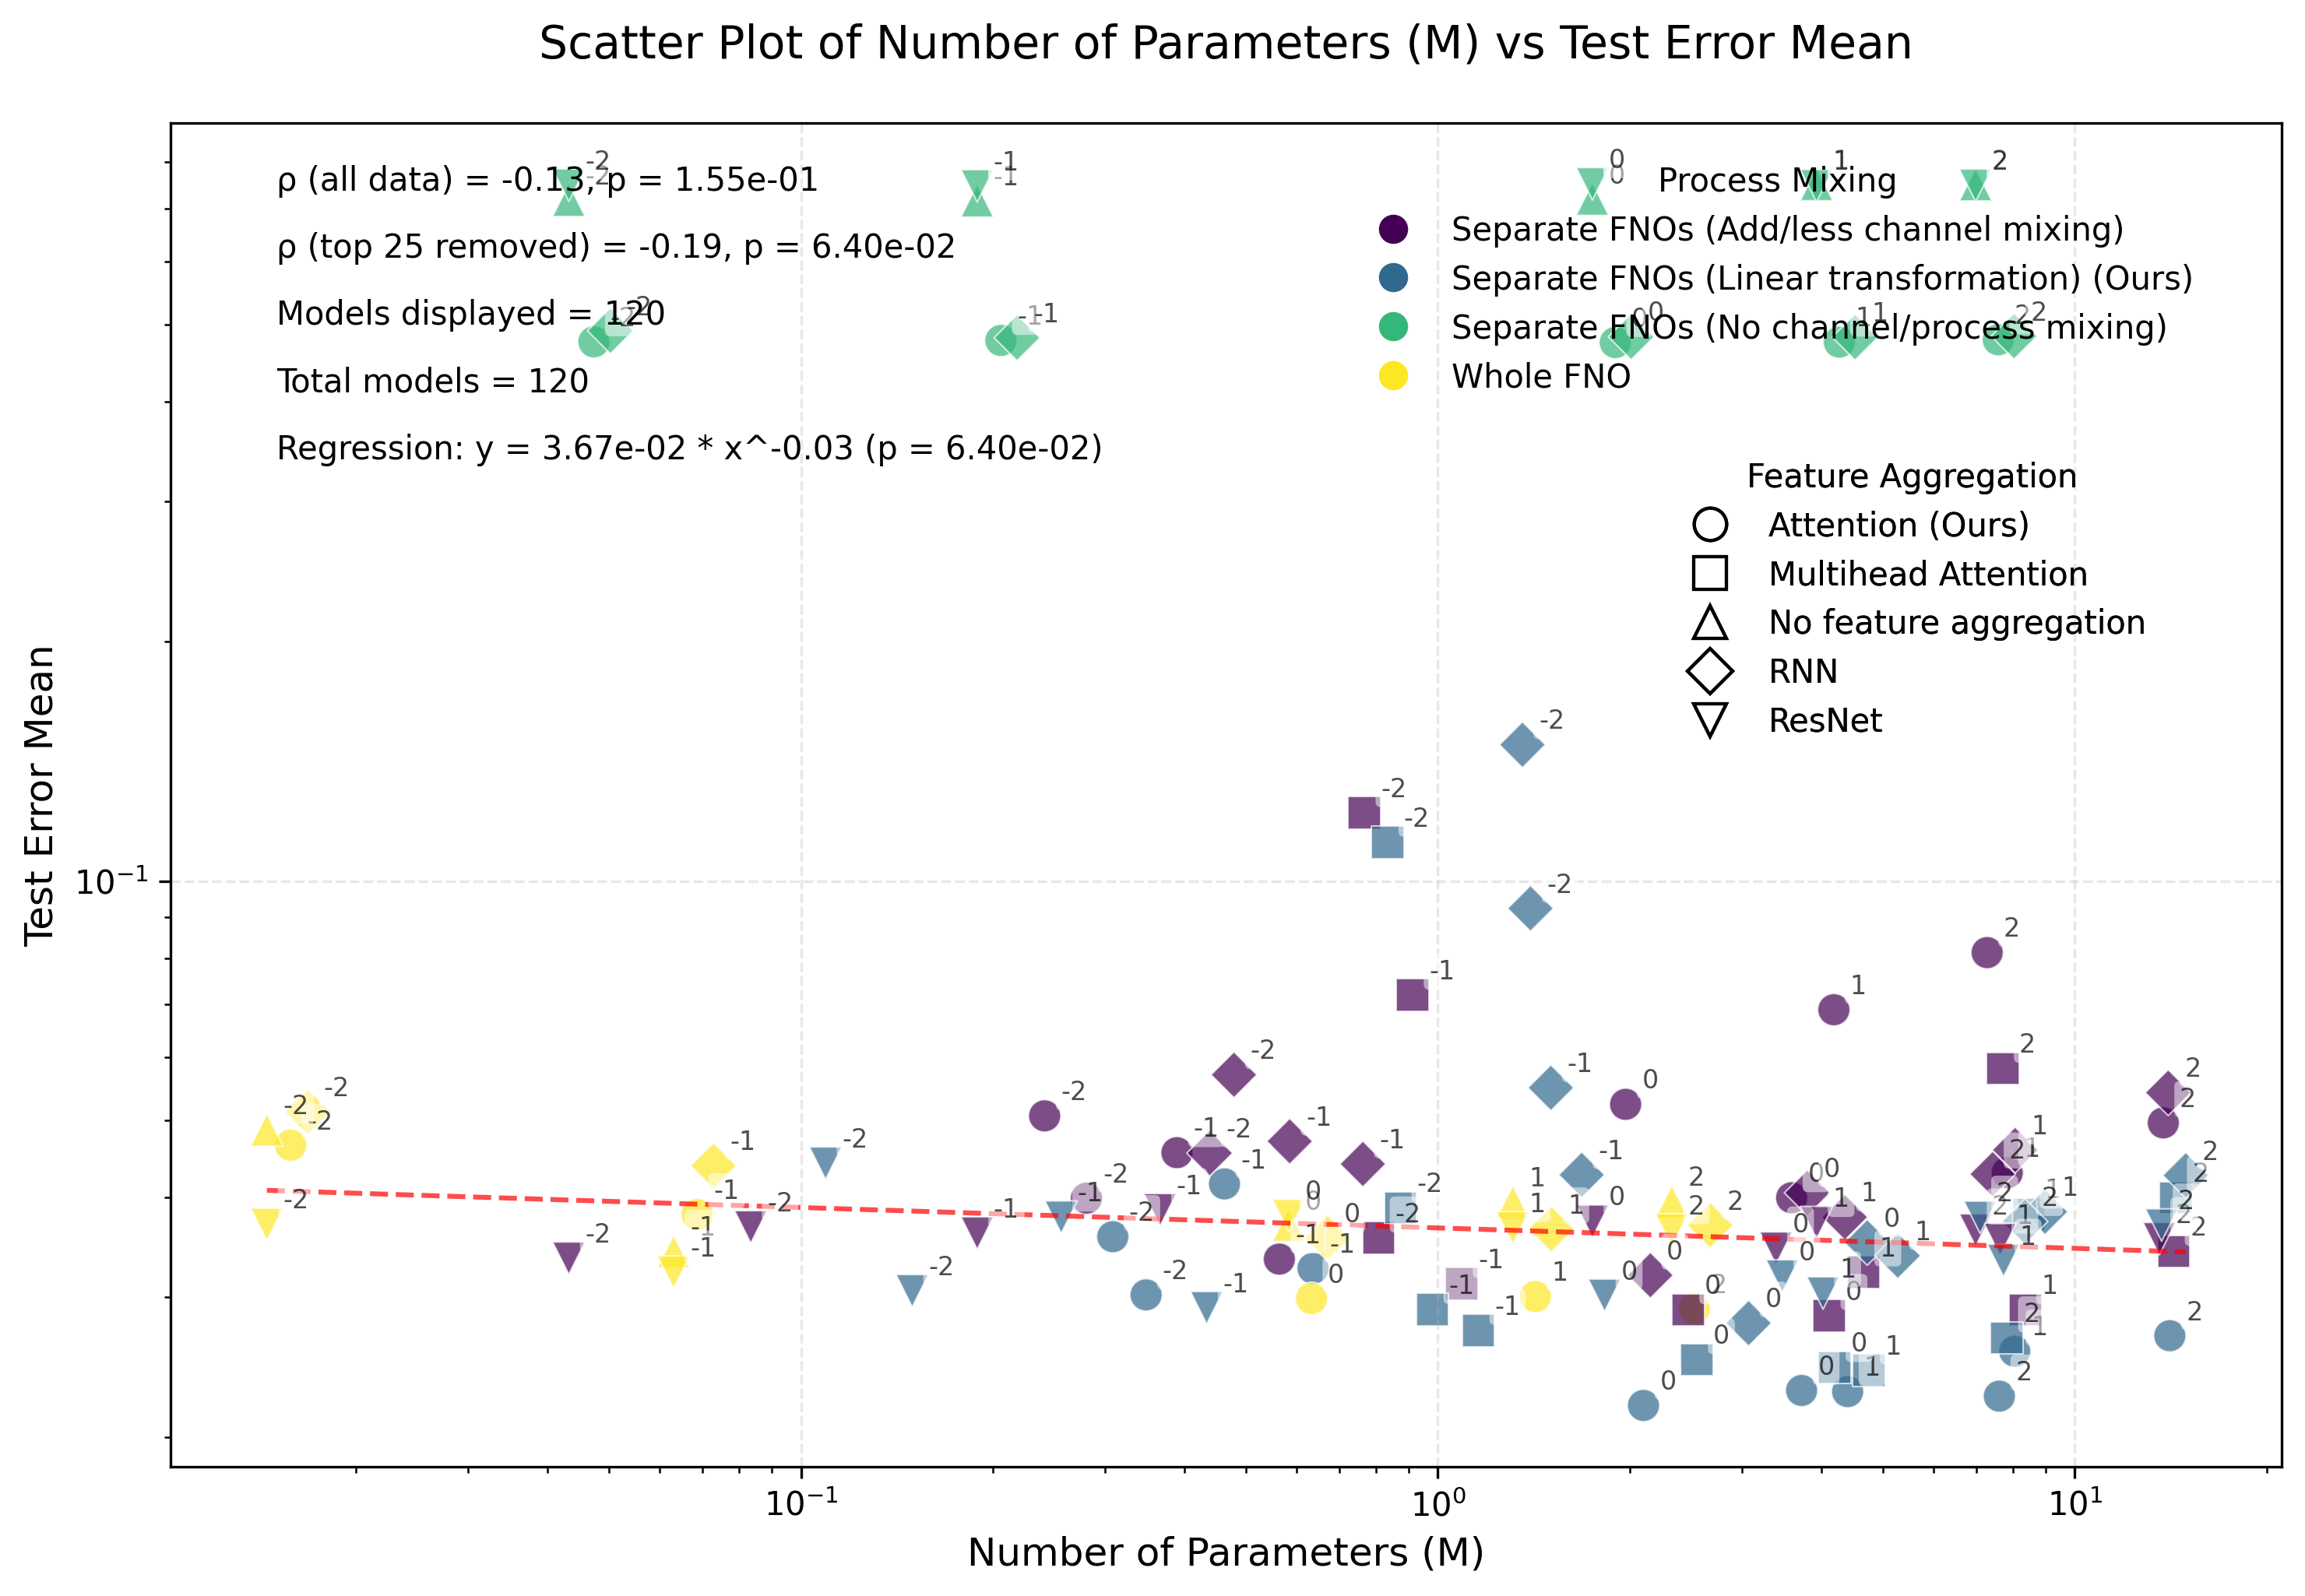
\includegraphics[width=1.0\textwidth]{figs/ablation_figs/BZ_512_params_vs_testerr.png}
	\caption{
		Test Errors vs Number of Parameters of Belousov-Zhabotinsky Using 512 Training Samples
	}
	\label{fig:BZ_512_params_vs_testerr}
\end{figure*}

\begin{figure*}[!htbp]
	\centering
	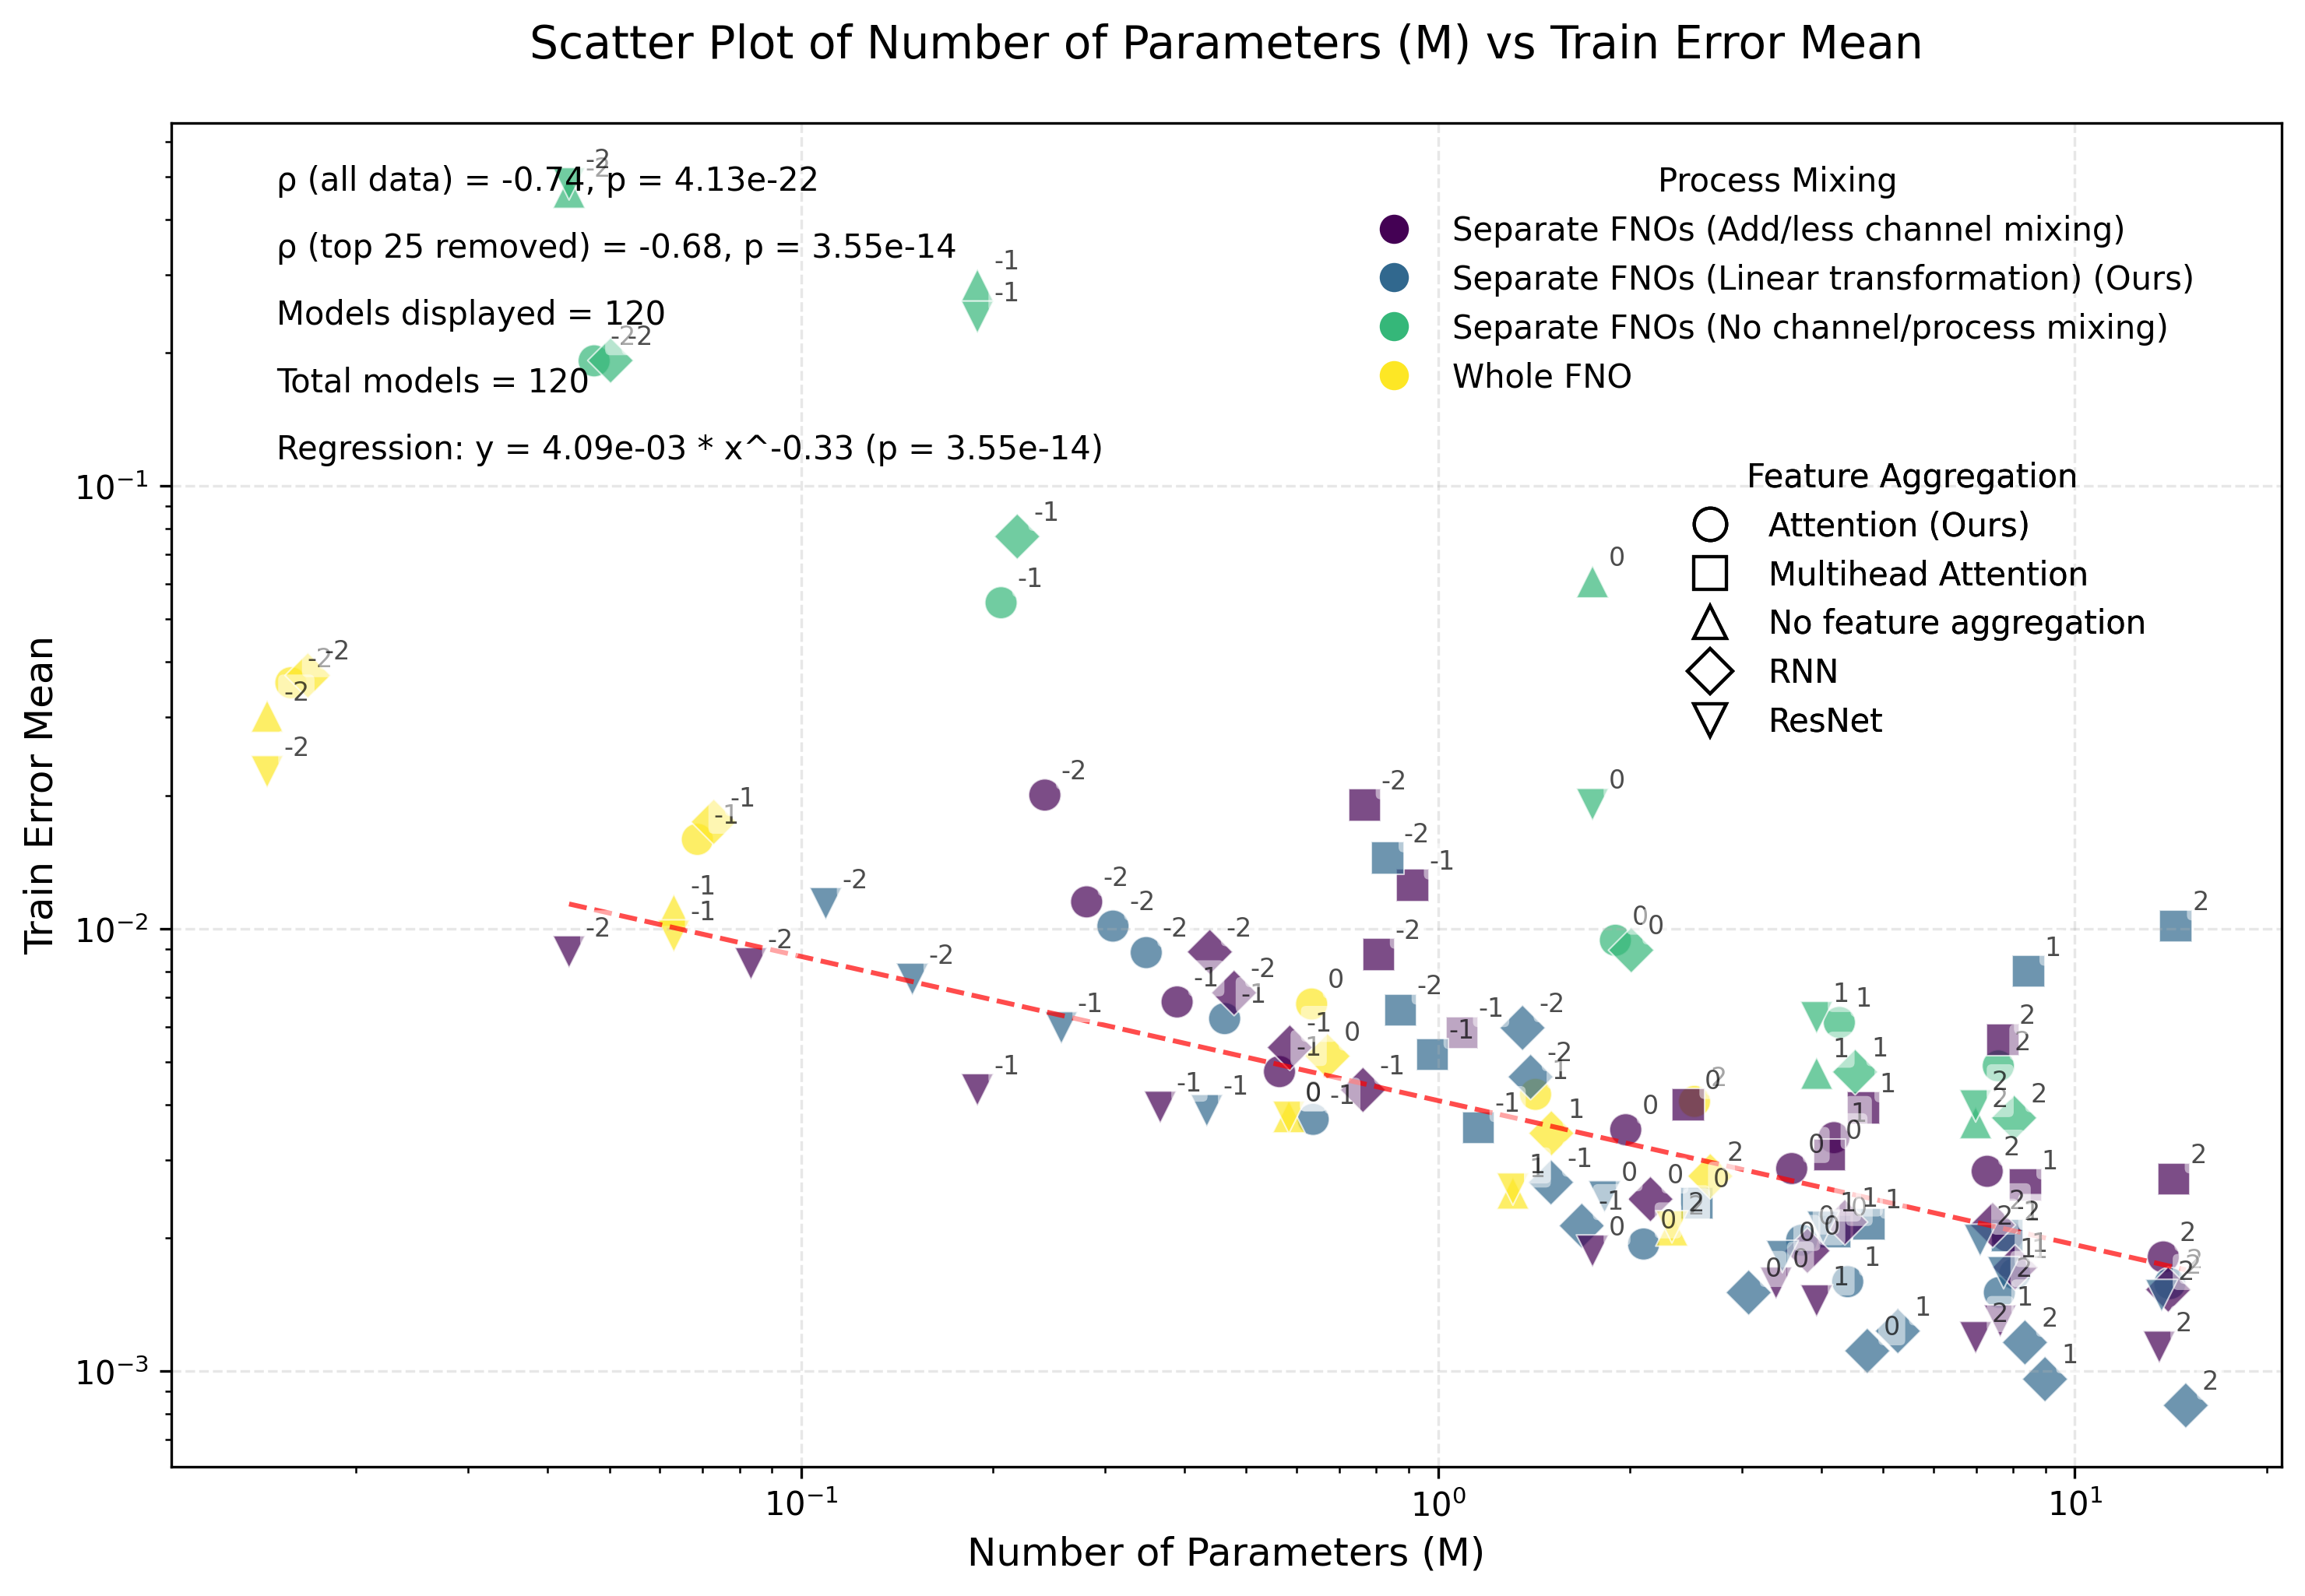
\includegraphics[width=1.0\textwidth]{figs/ablation_figs/BZ_512_params_vs_trainerr.png}
	\caption{
		Test Errors vs Number of Parameters of Belousov-Zhabotinsky Using 512 Training Samples
	}
	\label{fig:BZ_512_params_vs_trainerr}
\end{figure*}

\begin{figure*}[!htbp]
	\centering
	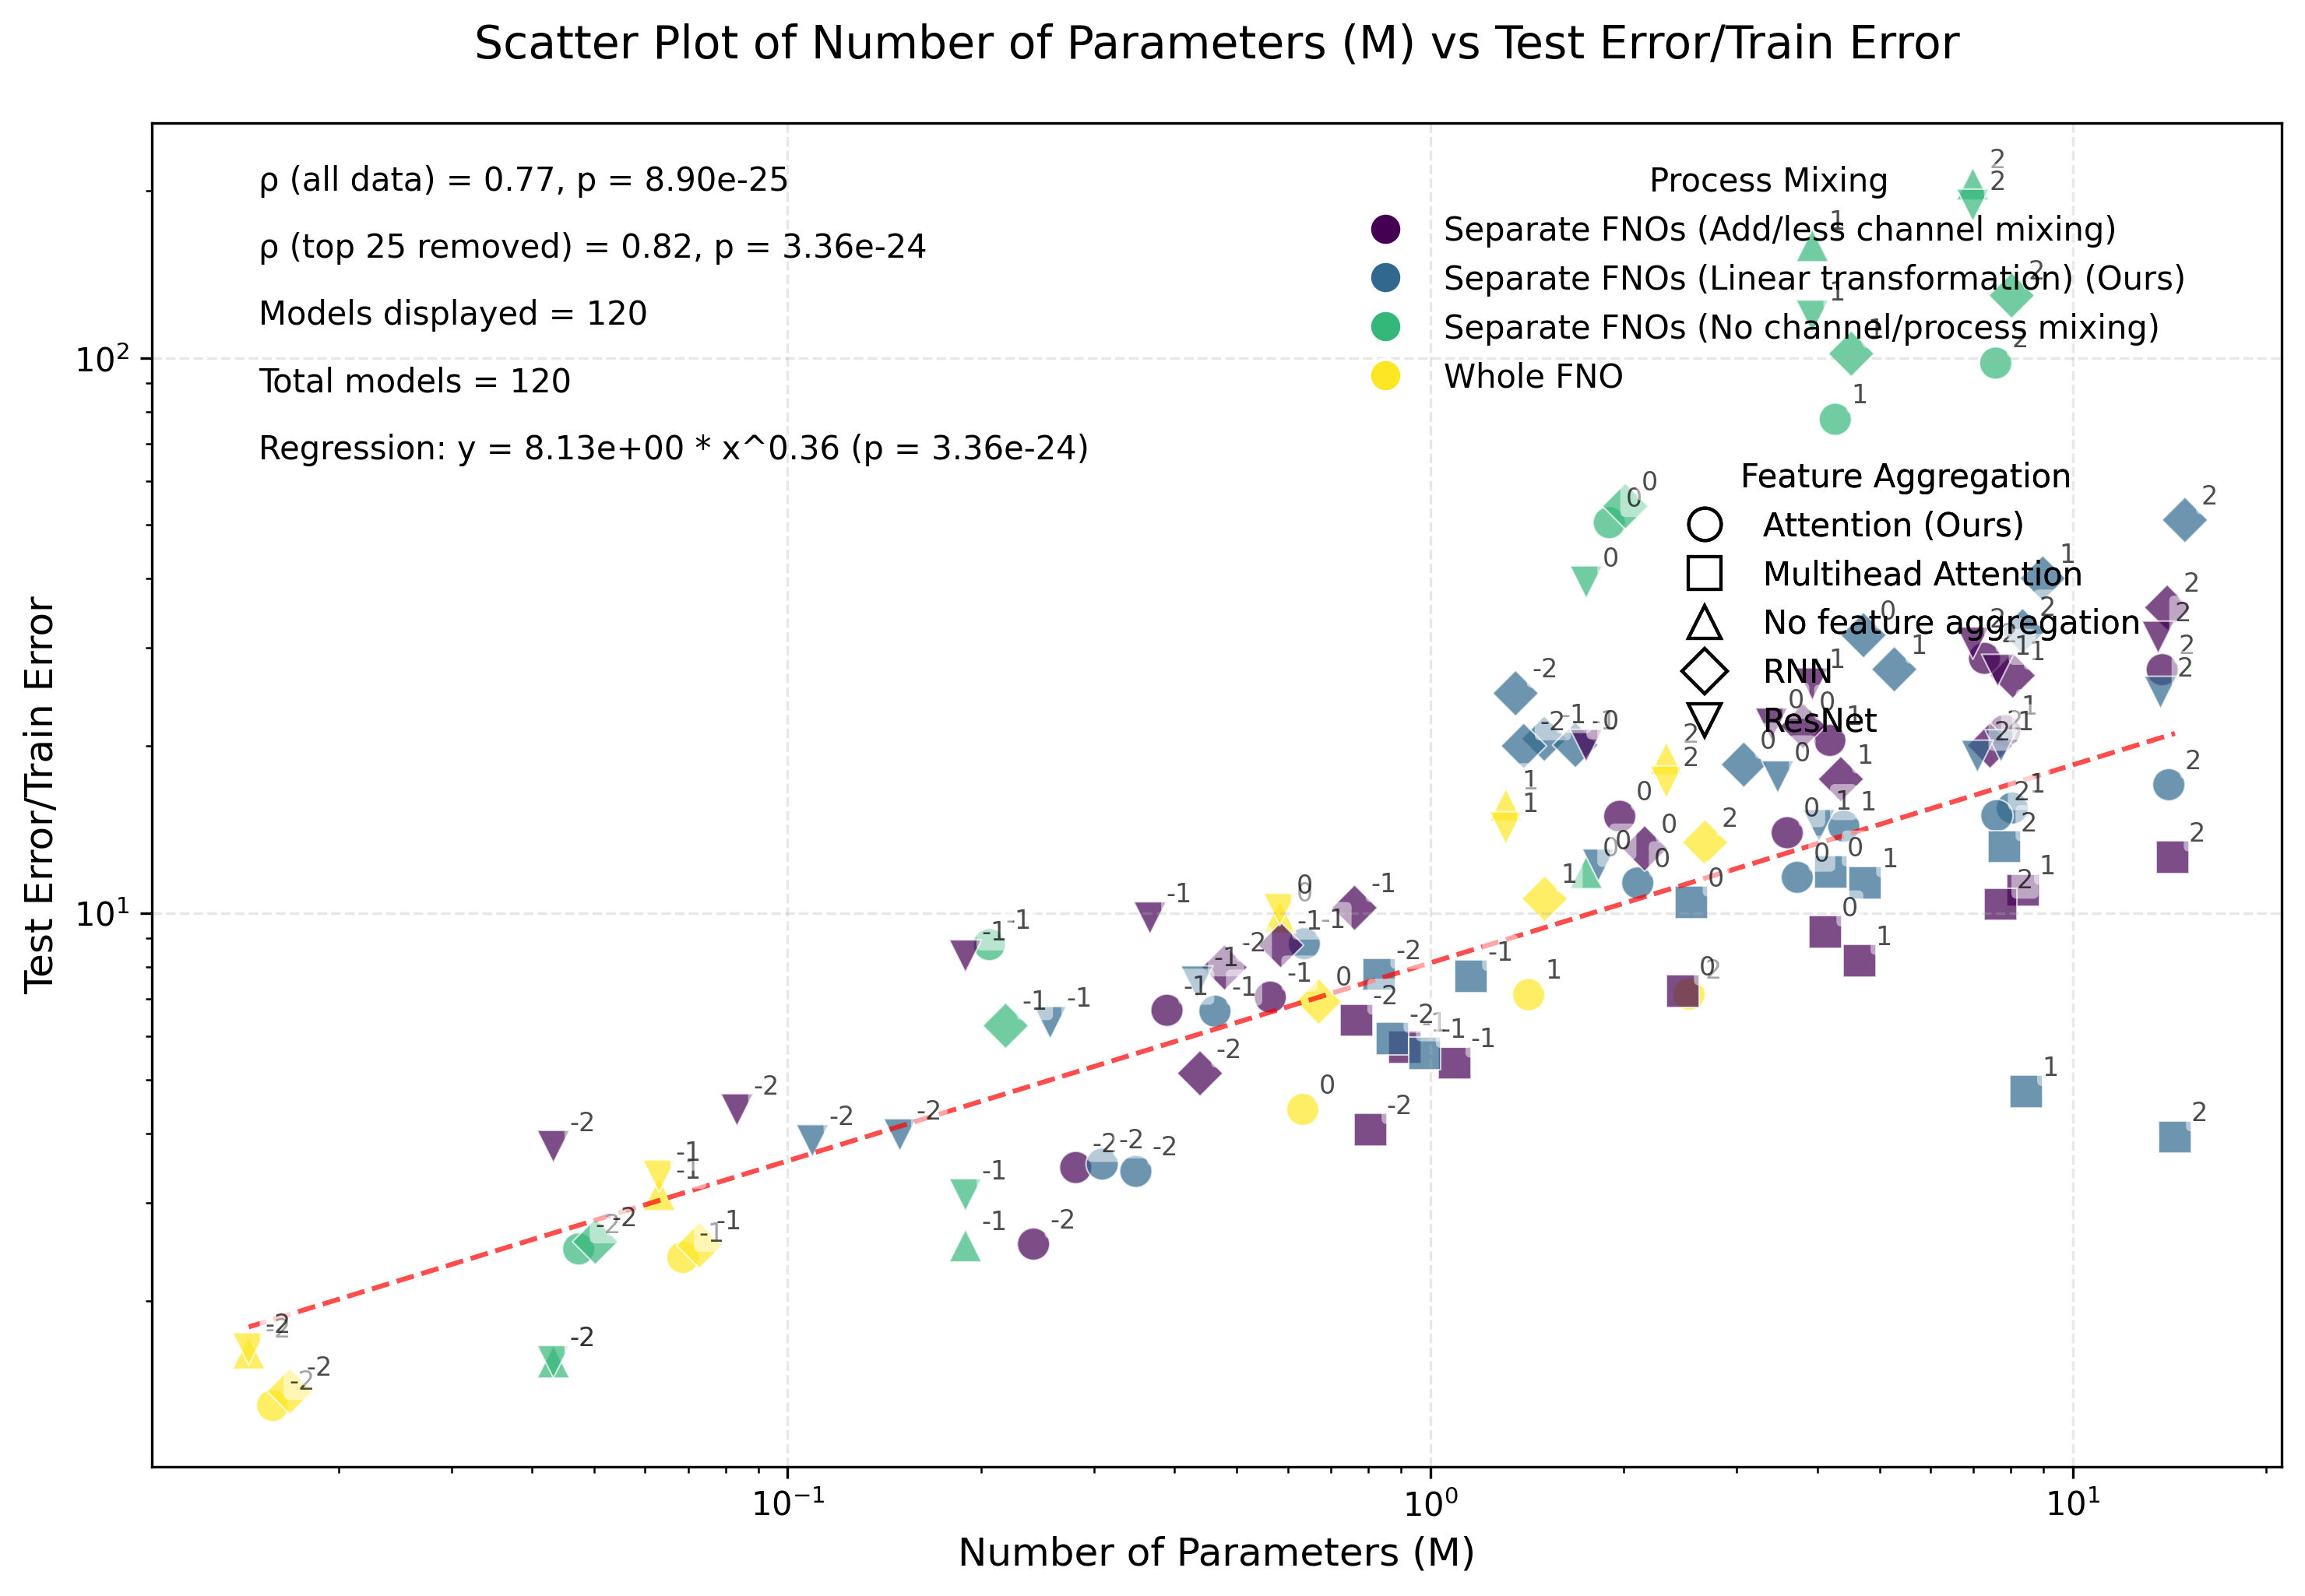
\includegraphics[width=1.0\textwidth]{figs/ablation_figs/BZ_512_params_vs_testtrainratio.png}
	\caption{
		Test Errors Over Train Errors Ratio vs Number of Parameters of Belousov-Zhabotinsky Using 512 Training Samples
	}
	\label{fig:BZ_512_params_vs_testtrainratio}
\end{figure*}




\begin{figure*}[!htbp]
	\centering
	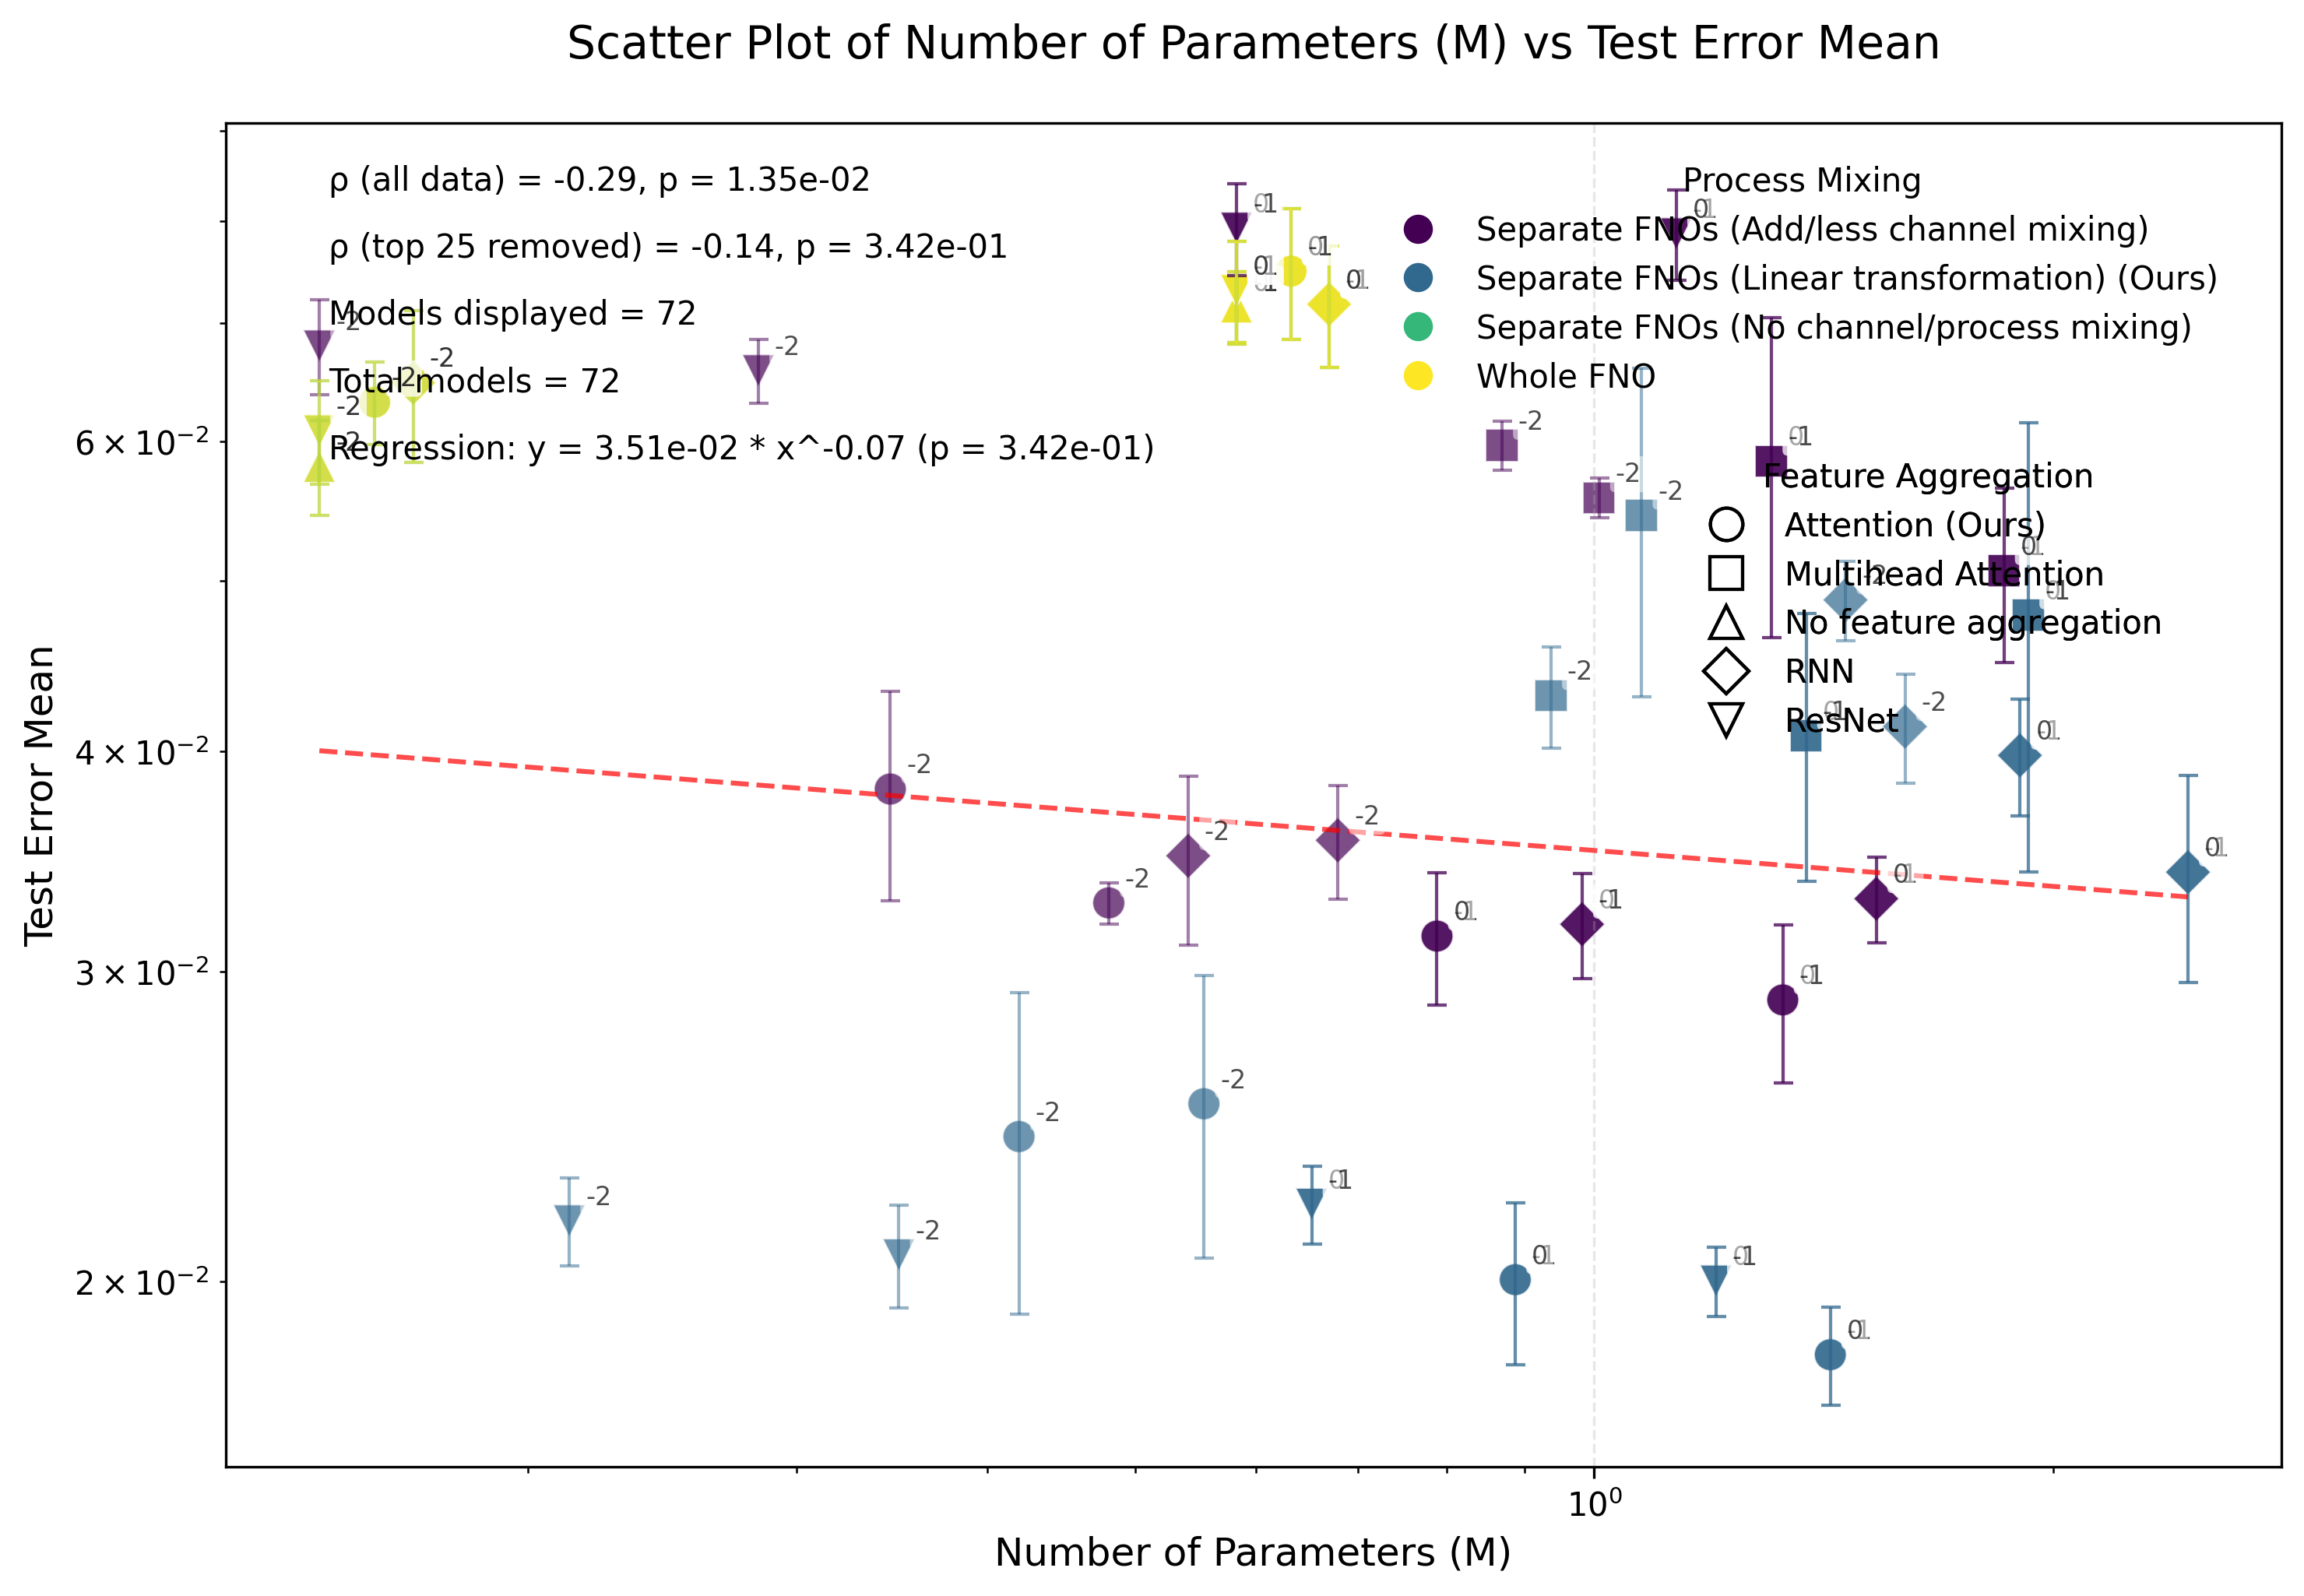
\includegraphics[width=1.0\textwidth]{figs/ablation_figs/Burgers_512_params_vs_testerr.png}
	\caption{
		Test Errors vs Number of Parameters of Burgers Using 512 Training Samples
	}
	\label{fig:Burgers_512_params_vs_testerr}
\end{figure*}

\begin{figure*}[!htbp]
	\centering
	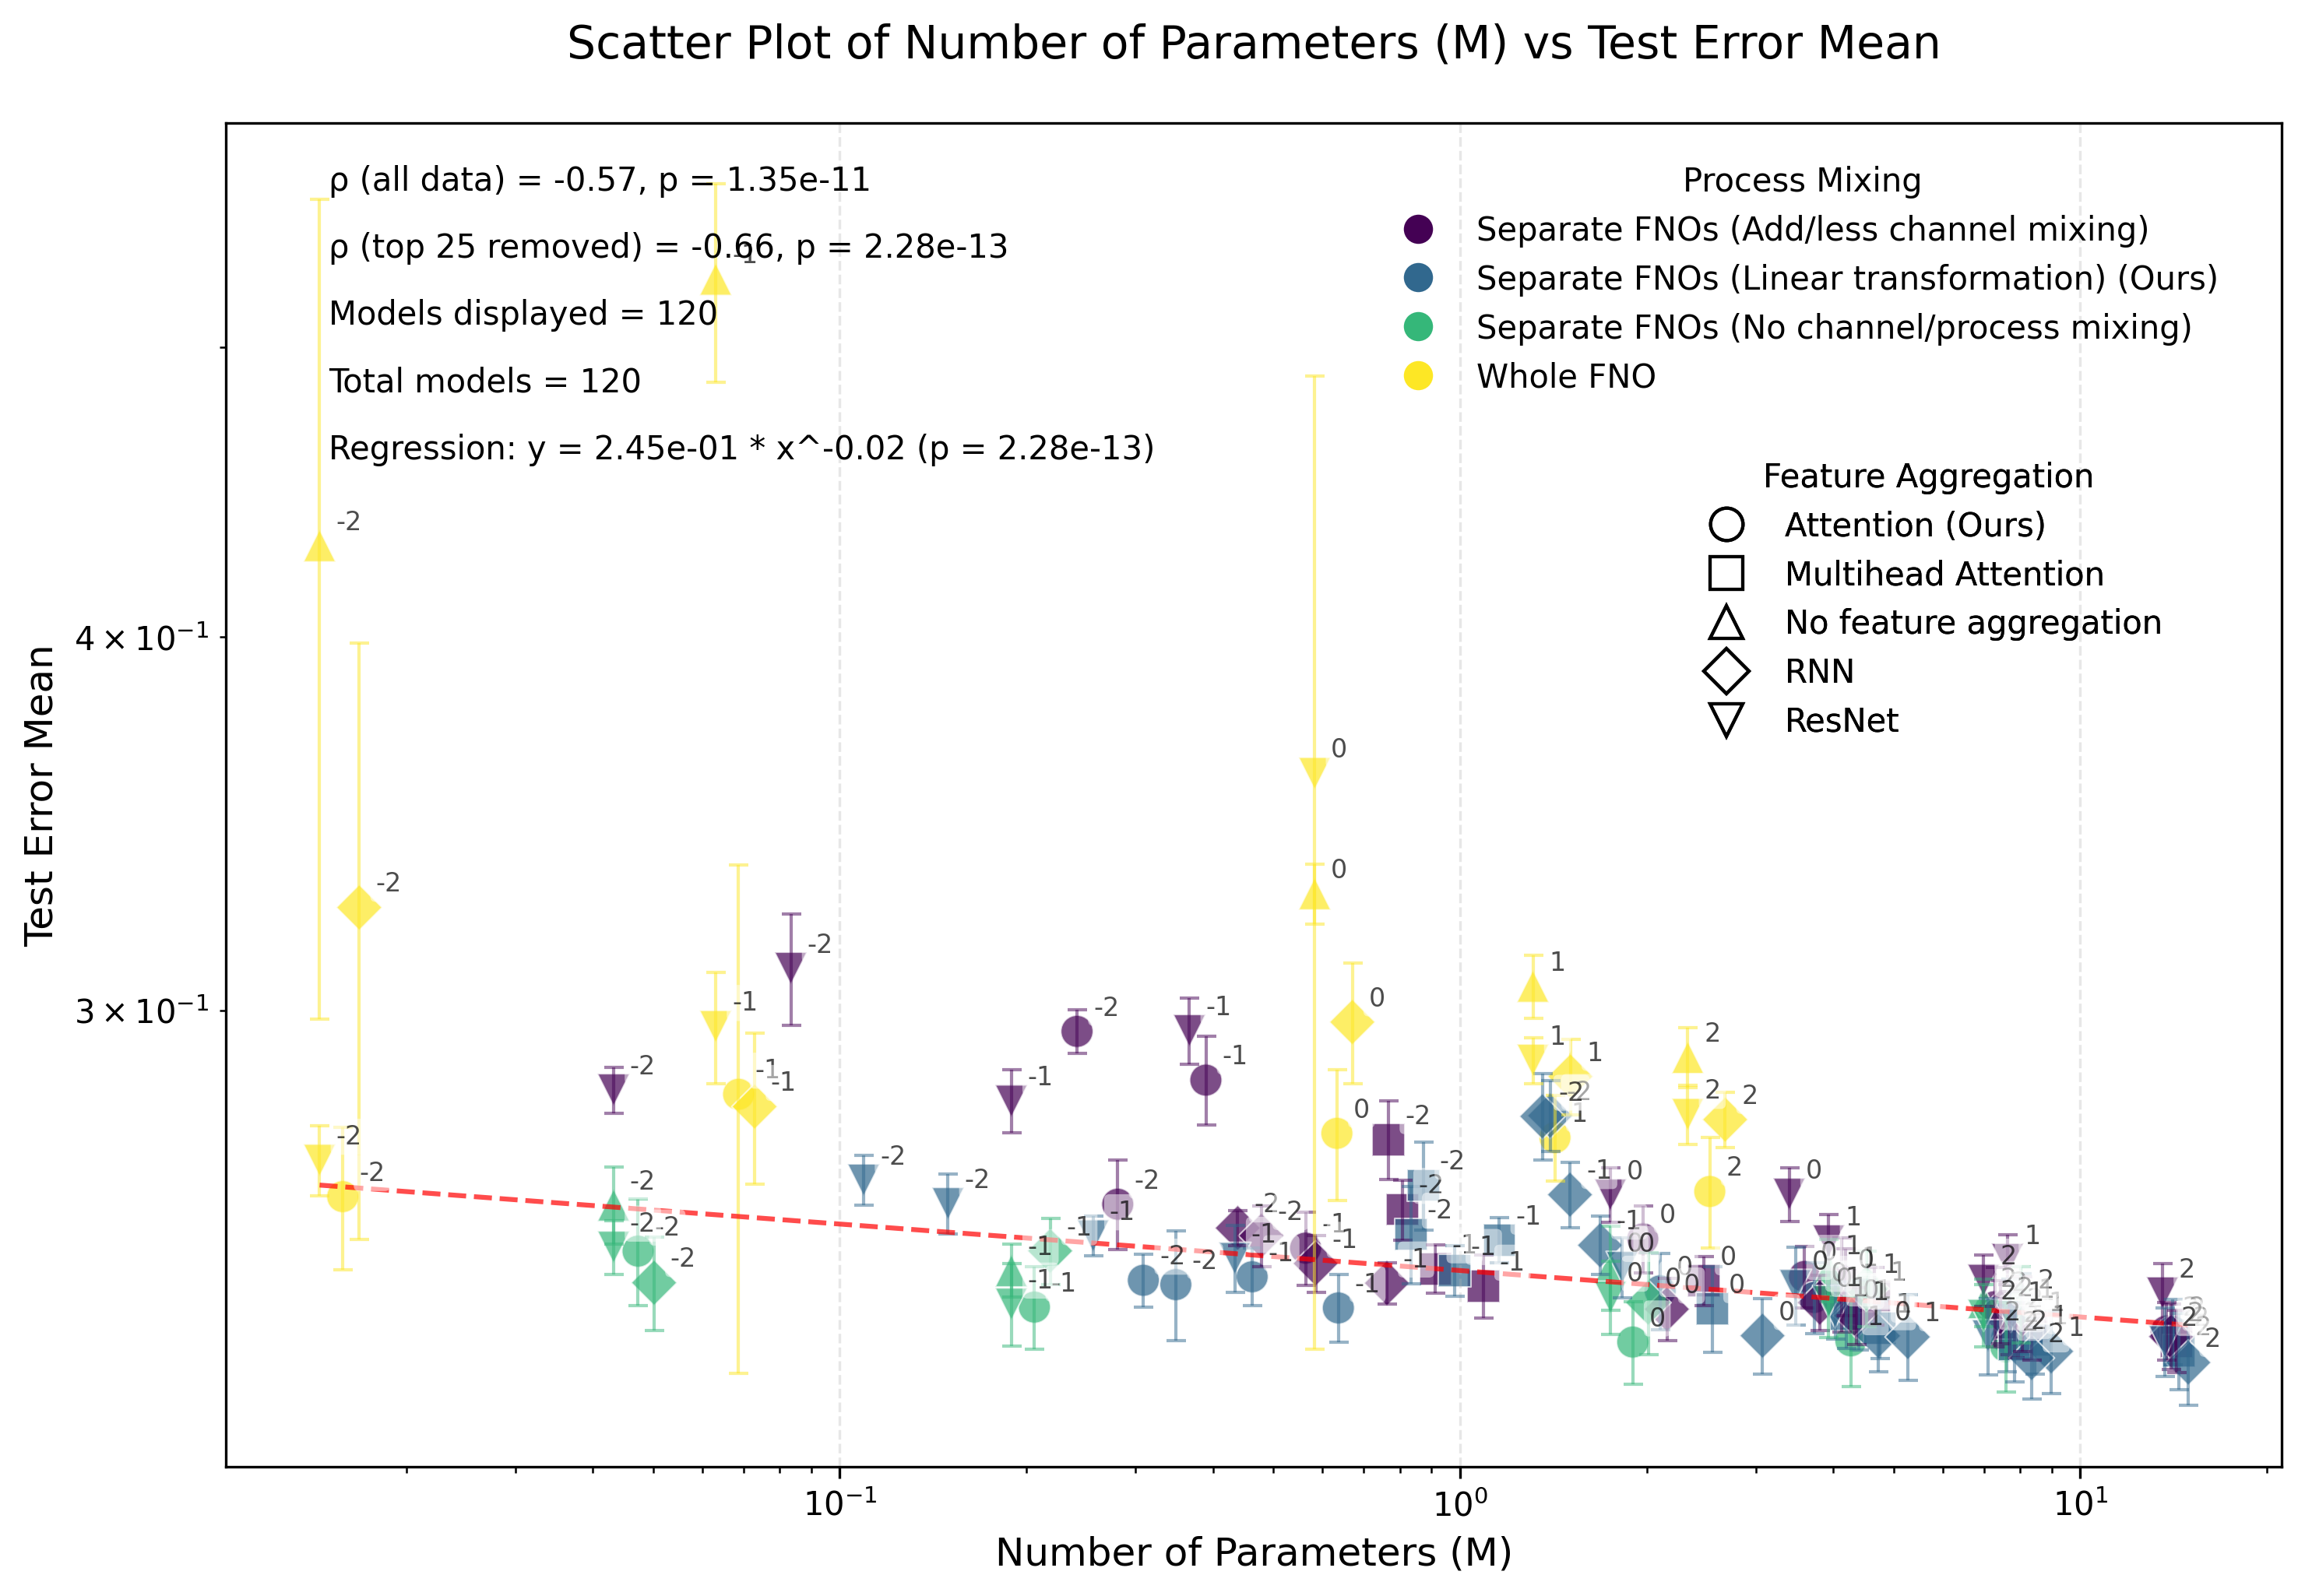
\includegraphics[width=1.0\textwidth]{figs/synthetic/synthetic_params_vs_testerr.png}
	\caption{
		Test Errors vs Number of Parameters of Our Synthetic Test Case from BZ, LV and Burgers Using 512 Training Samples
	}
	\label{fig:synthetic_512_params_vs_testerr}
\end{figure*}



\begin{figure*}[!htbp]
	\centering
	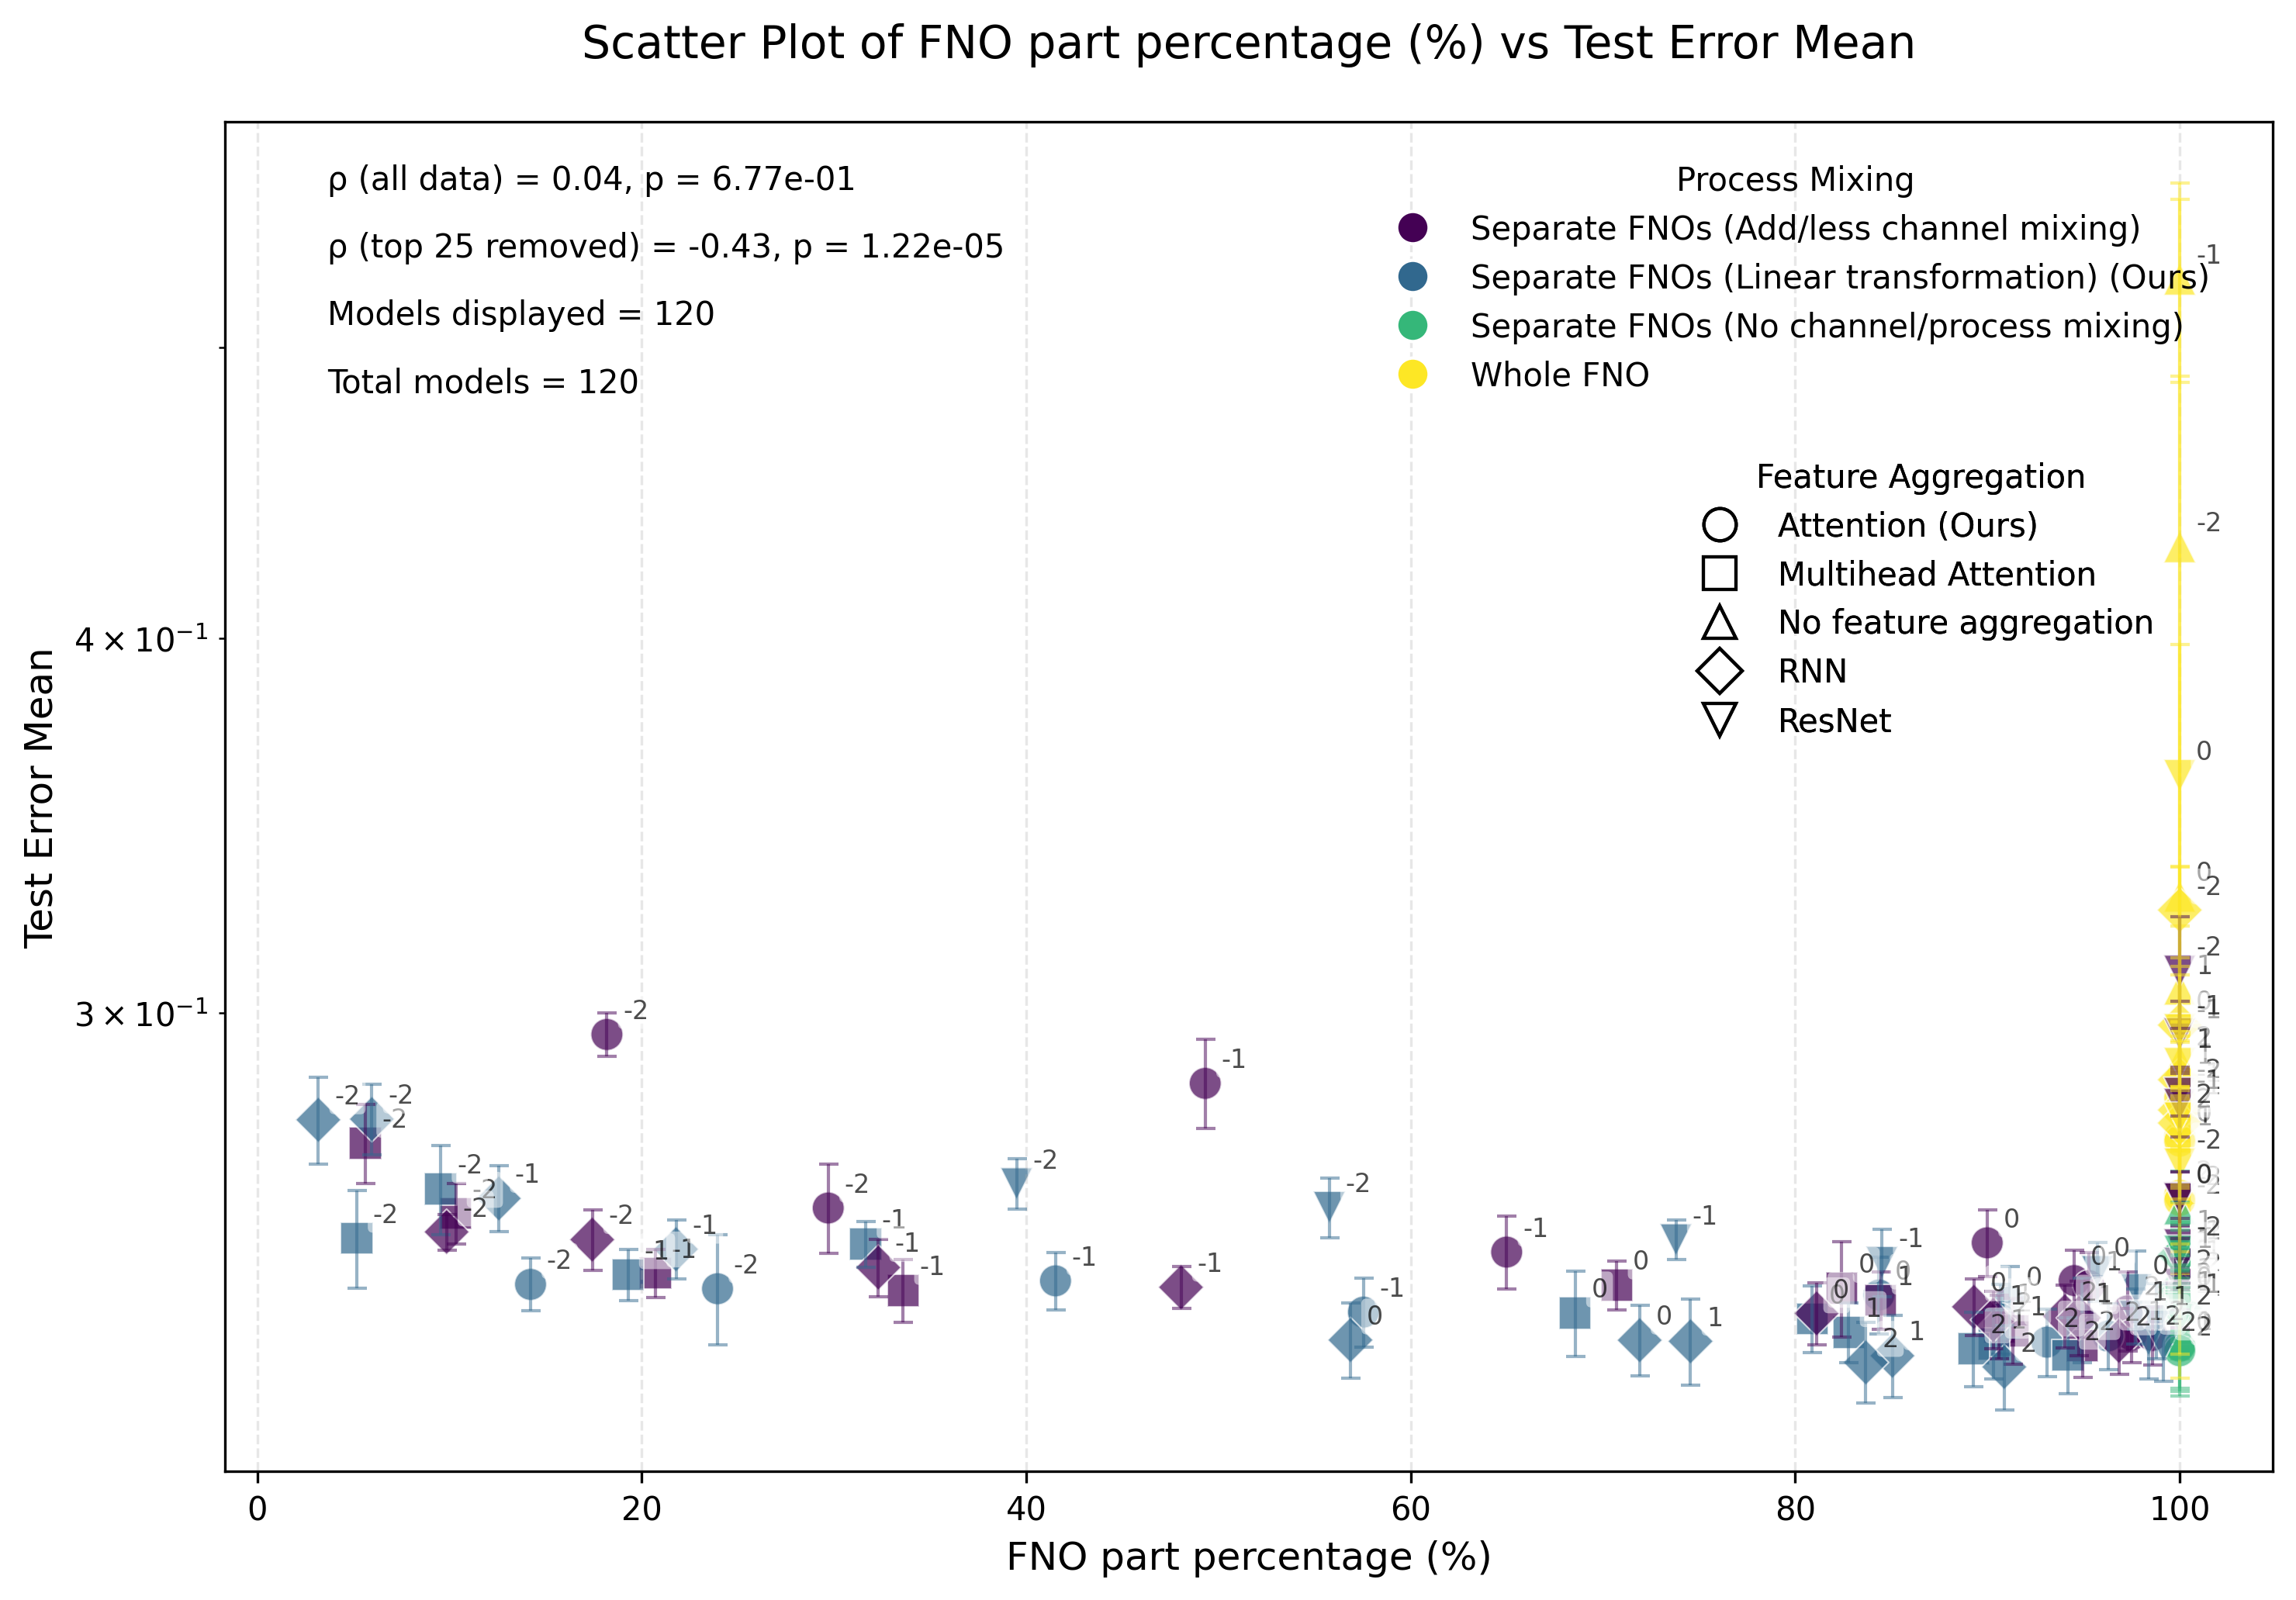
\includegraphics[width=1.0\textwidth]{figs/synthetic/synthetic_FNOperc_vs_testerr.png}
	\caption{
		Test Errors vs Percentage of FNO Parameters of Our Synthetic Test Case from BZ, LV and Burgers Using 512 Training Samples
	}  
	\label{fig:synthetic_512_FNOperc_vs_testerr}
\end{figure*}











